\documentclass[pdf]{beamer}
\mode<presentation>{}
\usepackage{minted}
\usepackage{tikz}
\usepackage{pgffor} %% gives looping with \foreach
\usepackage[absolute,overlay]{textpos}
\usepackage{lmodern} %% scalable latin characters
\usetikzlibrary{arrows,shapes,backgrounds}
\usepackage{multirow}
\usepackage{listings} %% another package for code related stuff

%% stuff for minted
\definecolor{mintedBg}{rgb}{0.95, 0.95, 0.95}
\definecolor{blockBg}{rgb}{0.6, 0.6, 0.95}
\definecolor{rnaColor}{rgb}{0, 0.6, 0}
\definecolor{cdsColor}{rgb}{0, 0.4, 0.4}
\definecolor{rnaPol}{rgb}{0.8,0,0.8}
\definecolor{ribosomeCol}{rgb}{0.5,0.5,0.1}
\definecolor{protColor}{rgb}{0.6,0,0.6}
%% colours for nucleotides:
\definecolor{dACol}{rgb}{0.5, 0.5, 0}
\definecolor{dCCol}{rgb}{0.8, 0, 0}
\definecolor{dGCol}{rgb}{0, 0.8, 0}
\definecolor{dTCol}{rgb}{0, 0, 0.8}

\definecolor{navy}{rgb}{0, 0, 0.6}
\definecolor{pur}{rgb}{0, 0, 0.6}
\definecolor{pyr}{rgb}{0.6, 0, 0.2}
%% define styles for different codes
\newminted{cpp}{linenos, bgcolor=blockBg, fontsize=\footnotesize}
%% then use \begin{cppcode}
\newminted{c}{linenos, bgcolor=mintedBg, fontsize=\footnotesize}
\newminted{perl}{linenos, bgcolor=mintedBg, fontsize=\footnotesize}

%% a command to define a subheading
\newcommand\subHeading[1]{
  \par\bigskip {\Large\bfseries#1}\par\smallskip
}

%% I detest indentation in footnotes etc, so try this:
\makeatletter
\renewcommand\@makefntext[1]{\noindent\makebox[0em][r]{\@makefnmark}\tiny#1}
\makeatother
%% the makeatletter and makeatother are required to allow me to
%% to change the macro beginning with an @. (though when I call it
%% I don't use the @ ... 

\setlength\parskip{0.5em}
\setlength\parindent{0ex}

%% to have footnotes without references. This from tex.stackexchange.com
\newcommand\blfootnote[1]{%
  \begingroup  %% this makes it a local redefinition
  \renewcommand\thefootnote{}\footnote{#1}%
  \addtocounter{footnote}{-1}  % this adjusts the footnote counter
  \endgroup
}


\title{Pairwise alignment}
\subtitle{basic alignment}
\author{Martin Jakt}

\begin{document}

\begin{frame}
  \titlepage
\end{frame}

\begin{frame}[fragile]{Why align (two) sequences?}
\begin{figure}[ht]
  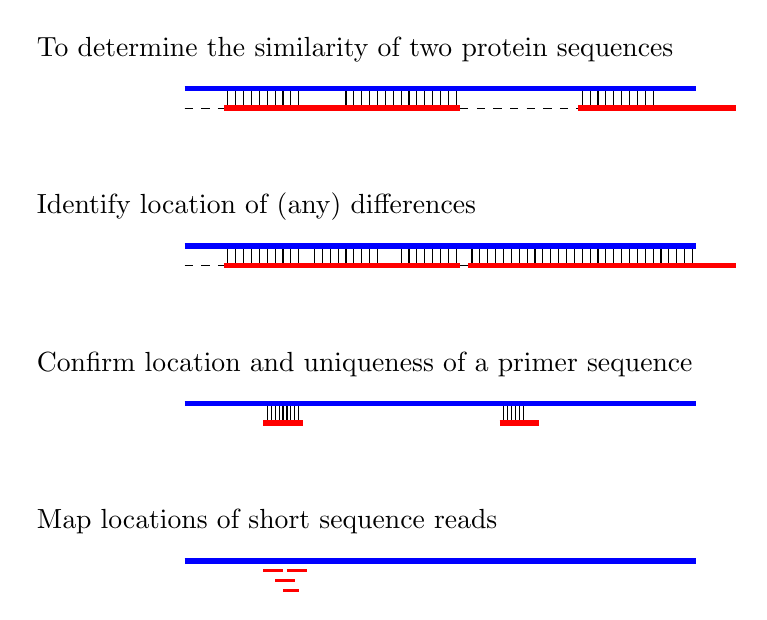
\begin{tikzpicture}[scale=0.5]
    %% \draw [help lines, opacity=1] (0,0) grid (22,12);
    %% \foreach \x in {1,2,...,19} \node [font=\small] at (\x,0) {\x};
    %% \foreach \y in {1,2,...,18} \node [font=\small] at (20,\y) {\y};
    
    \visible<2->{
      \node [right, align=left] at (1,18) {To determine the similarity of two
        protein sequences};
      \foreach \x in {6.1,6.3,...,7.9} \draw [-] (\x,17) -- (\x,16.5);
      \foreach \x in {9.1,9.3,...,11.9} \draw [-] (\x,17) -- (\x,16.5);
      \foreach \x in {15.1,15.3,...,16.9} \draw [-] (\x,17) -- (\x,16.5);
      
      \draw [-, line width=2,blue] (5,17) -- (18,17);
      \draw [-, dashed] (5,16.5) -- (6,16.5);
      \draw [-, dashed] (5,16.5) -- (6,16.5);
      \draw [-, line width=2,red] (6,16.5) -- (12,16.5);
      \draw [-, dashed] (12,16.5) -- (15,16.5);
      \draw [-, line width=2,red] (15,16.5) -- (19,16.5);
    }
    \visible<3->{
      \node [right, align=left] at (1,14) {Identify location of (any)
        differences};

      \foreach \x in {6.1,6.3,...,7.9} \draw [-] (\x,13) -- (\x,12.5);
      \foreach \x in {8.3,8.5,...,9.9} \draw [-] (\x,13) -- (\x,12.5);
      \foreach \x in {10.5,10.7,...,11.9} \draw [-] (\x,13) -- (\x,12.5);
      \foreach \x in {12.3,12.5,...,17.9} \draw [-] (\x,13) -- (\x,12.5);
      
      \draw [-, dashed] (5,12.5) -- (6,12.5);
      \draw [-, line width=2,blue] (5,13) -- (18,13);
      \draw [-, line width=2,red] (6,12.5) -- (12,12.5);
      \draw [-, line width=2,red] (12.2,12.5) -- (19,12.5);
      \draw [-, dashed] (12,12.5) -- (12.2,12.5);

    }
    \visible<4->{
      \node [right, align=left] at (1,10) {Confirm location and uniqueness of a
        primer sequence};
      
      \foreach \x in {7.1, 7.2,...,7.9} \draw [-] (\x,9) -- (\x,8.5);
      \foreach \x in {13.1, 13.2,...,13.6} \draw [-] (\x,9) -- (\x,8.5);
      \draw [-, line width=2,blue] (5,9) -- (18,9);
      \draw [-, line width=2,red] (7,8.5) -- (8,8.5);
      \draw [-, line width=2, red] (13,8.5) -- (14,8.5);
      
    }
    \visible<5->{
      \node [right, align=left] at (1,6) {Map locations of short sequence
        reads};
      \draw [-, line width=2,blue] (5,5) -- (18,5);
      \draw [-, line width=1,red] (7,4.75) -- (7.5,4.75);
      \draw [-, line width=1,red] (7.6,4.75) -- (8.1,4.75);
      \draw [-, line width=1,red] (7.3,4.5) -- (7.8,4.5);
      \draw [-, line width=1,red] (7.5,4.25) -- (7.9,4.25);
    }
  \end{tikzpicture}
\end{figure}
\end{frame}



\begin{frame}[fragile]{A simple alignment}
  The two following sequences have an obvious alignment.
  \begin{verbatim}
    TAATTAGC
    CATTA
  \end{verbatim}
  \begin{figure}[ht]
  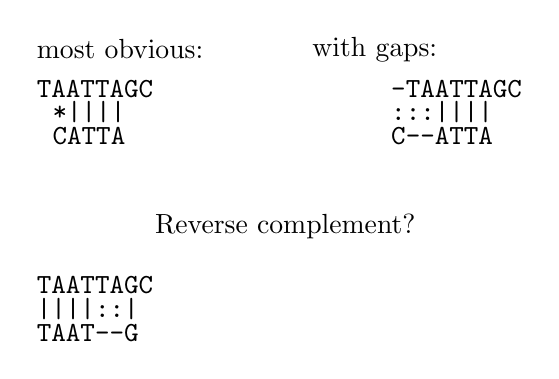
\begin{tikzpicture}[scale=0.5]
%    \draw [help lines, opacity=1] (0,0) grid (22,12);
%    \foreach \x in {1,2,...,19} \node [font=\small] at (\x,0) {\x};
%    \foreach \y in {1,2,...,12} \node [font=\small] at (20,\y) {\y};
    \visible<2->{
      \node [right, align=left] at (1,12) {most obvious:};
      \node [right, font=\ttfamily] at (1., 11)   {TAATTAGC};
      \node [right, font=\ttfamily] at (1.4,10.4) { *||||}; 
      \node [right, font=\ttfamily] at (1.4,9.8)  { CATTA}; 
    }
    \visible<3->{
      \node [right, align=left] at (8,12) {with gaps:};
      \node [right, font=\ttfamily] at (10,11)   {-TAATTAGC};
      \node [right, font=\ttfamily] at (10,10.4) {:::||||};
      \node [right, font=\ttfamily] at (10,9.8)  {C--ATTA};
    }
    \visible<4->{
      \node [right, align=left] at (4,7.5) {Reverse complement?};
      \node [right, align=left, font=\ttfamily] at (1,6)   {TAATTAGC};
      \node [right, align=left, font=\ttfamily] at (1,5.4) {||||::|};
      \node [right, align=left, font=\ttfamily] at (1,4.8) {TAAT--G};
    }
  \end{tikzpicture}
\end{figure}
\visible<5->{
  Which is the best alignment?\\
  Depends on the question asked.
}
\end{frame}

\begin{frame}[fragile]{Different types of alignment}
  \begin{figure}[ht]
    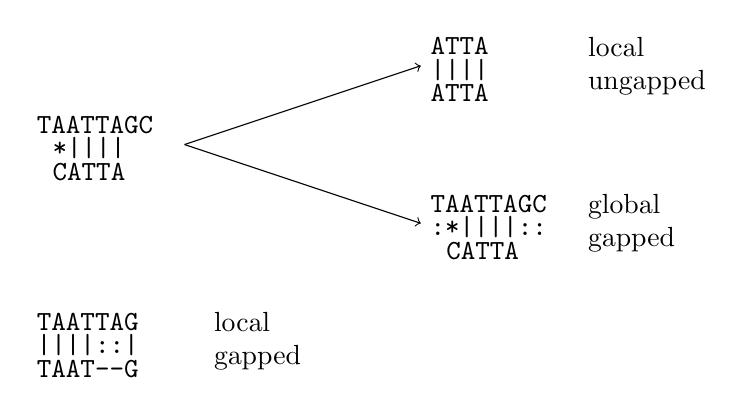
\begin{tikzpicture}[scale=0.5]
      %% \draw [help lines, opacity=1] (0,0) grid (22,12);
      %% \foreach \x in {1,2,...,19} \node [font=\small] at (\x,0) {\x};
      %% \foreach \y in {1,2,...,12} \node [font=\small] at (20,\y) {\y};
      \visible<2->{
        \node [right, font=\ttfamily] at (1., 11)   {TAATTAGC};
        \node [right, font=\ttfamily] at (1.4,10.4) { *||||}; 
        \node [right, font=\ttfamily] at (1.4,9.8)  { CATTA}; 
      }
      \visible<3->{
        \draw[->] (5, 10.5) -- (11,12.5);
        \node [right, font=\ttfamily] at (11., 13)   {ATTA};
        \node [right, font=\ttfamily] at (11.,12.4) {||||}; 
        \node [right, font=\ttfamily] at (11.,11.8)  {ATTA}; 
        \node [right, align=left] at (15,12.5) {local\\ungapped};
      }
      \visible<4->{
        \draw[->] (5, 10.5) -- (11,8.5);
        \node [right, font=\ttfamily] at (11., 9)   {TAATTAGC};
        \node [right, font=\ttfamily] at (11.,8.4) {:*||||::}; 
        \node [right, font=\ttfamily] at (11.4,7.8)  {CATTA}; 
        \node [right, align=left] at (15,8.5) {global\\gapped};

      }
      \visible<5->{
        \node [right, align=left, font=\ttfamily] at (1,6)   {TAATTAG};
        \node [right, align=left, font=\ttfamily] at (1,5.4) {||||::|};
        \node [right, align=left, font=\ttfamily] at (1,4.8) {TAAT--G};
        \node [right, align=left] at (5.5,5.5) {local\\gapped};
      }
    \end{tikzpicture}
  \end{figure}
\end{frame}

\begin{frame}{Different types of alignment (2)}
  \begin{description}
  \item[global] Includes all residues in both sequences. Must include gaps if
    unequal length.
  \item[local] Includes only the highest scoring sub alignment. May include
    more than one aligned region.
  \item[pseudo-global\footnote{May not be the correct term.}] Includes all residues from the shorter sequence. Not
    penalised for initial terminal gaps?!\footnote{We'll cover the meaning of
      these in more details when we look at the algorithms.}.
  \end{description}
\end{frame}

\begin{frame}{Evaluating an alignment (1)}
  To get a score for an alignment:
  \begin{enumerate}
  \item Assign a score or penalty for matches, mismatches, gaps.
  \item Add up the appropriate scores / penalties at each position in the
    alignment.
  \item The sum is the alignment score.
  \end{enumerate}
\end{frame}

\begin{frame}{Evaluating an alignment (2)}
  More formally:
  $$
  S_a =  (N_{m} \times P_m) + (N_{mm} \times P_{mm}) + (N_{gap} \times P_{gap})
  $$
  {\footnotesize
  Where
  \begin{description}
    \item[$N_{m}$] number of matches
    \item[$N_{mm}$] number mismatches
    \item[$N_{gap}$] number of gaps
    \item[$P_m$] penalty for a match
    \item[$P_{mm}$] penalty for a mismatch
    \item[$P_{gap}$] penalty for a gap
  \end{description}
  $P_{m}$, $P_{mm}$ and $P_{gap}$ can be tuned to favour different types of
  alignment. (A penalty can also be referred to as a cost or a score).

  \blfootnote{A penalty for a match is silly, but the equation looks nicer
    like this}
}
\end{frame}

\begin{frame}[fragile]{but too simple}
  Consider: \verb|ATTACTTAGGATTATAGA| and \verb|ATTAGATTA|
  \pause
  \begin{itemize}
  \item 
\begin{verbatim}
ATTACTTAGGATTATAGA
||   | | || | |  |
AT---T-A-GA-T-T--A
\end{verbatim} \pause
  \item
\begin{verbatim}
ATTACTTAGGATTATAGA
||||     |||||
ATTA-----GATTA----
\end{verbatim}
\end{itemize}
These will have the same scores, but the second alignment intuitively 'feels' better as:
\begin{itemize}
\item words can carry more meaning than individual letters
\item insertion deletion events are not restricted to single nucleotides
\end{itemize}
\end{frame}

\begin{frame}{Affine gap penalties}
Modify the alignment score:
%  $$
%  S_a =  N_{m} \times P_m + N_{mm} \times P_{mm}  + N_{go} \times P_{go} + N_{ge} \times P_{ge}
%  $$
  $$
  S_a =  N_{m}P_m + N_{mm}P_{mm}  + N_{go}P_{go} + N_{ge}P_{ge}
  $$

  where the penalties for gaps are divided into:
  \begin{itemize}
    \item initial gaps (gap opening) \hspace{4.75ex} $N_{go} \times P_{go}$
    \item successive gaps (gap extension) $N_{ge}\times P_{ge}$
  \end{itemize}
  \pause
  There are more complex alternatives (eg. the cost of extending a gap can
  be a function of the gap length), but a simple affine gap penalty is
  commonly used.

  For global alignments one can also consider terminal gaps differently
  (esp. if there is a difference in sequence lengths, necessitating terminal gaps).
\end{frame}

\begin{frame}[fragile]{Affine gap penalties (2)}
    \begin{figure}[ht]
      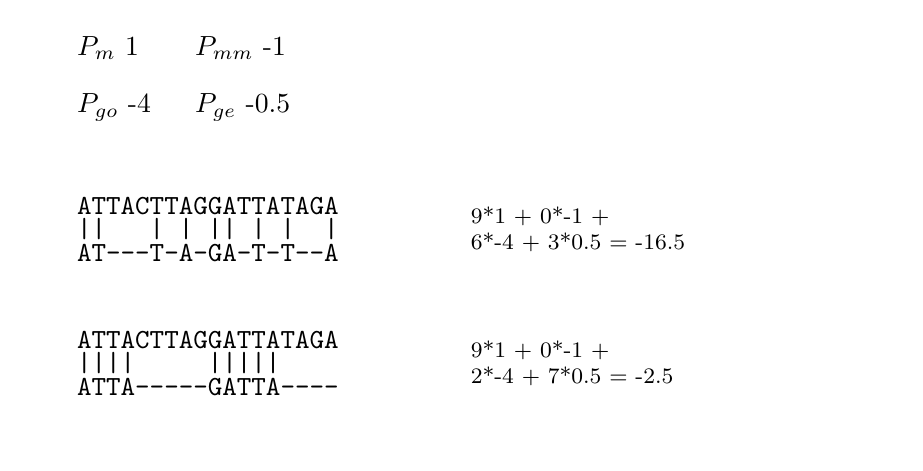
\begin{tikzpicture}[scale=0.5]
        \draw [help lines, opacity=0] (0,0) grid (22,10);
%        \foreach \x in {1,2,...,19} \node [font=\small] at (\x,0) {\x};
%        \foreach \y in {1,2,...,10} \node [font=\small] at (20,\y) {\y};
        \node [right] at (1,10) {$P_m$ 1};
        \node [right] at (4,10) {$P_{mm}$ -1};
        \node [right] at (1,8.5) {$P_{go}$ -4};
        \node [right] at (4,8.5) {$P_{ge}$ -0.5};
        \node [right, align=left, font=\ttfamily] at (1,6)   {\verb'ATTACTTAGGATTATAGA'};
        \node [right, align=left, font=\ttfamily] at (1,5.4) {\verb'||   | | || | |  |'};
        \node [right, align=left, font=\ttfamily] at (1,4.8) {\verb'AT---T-A-GA-T-T--A'};
        \node [right, align=left, font=\ttfamily] at (1,2.6) {\verb'ATTACTTAGGATTATAGA'};
        \node [right, align=left, font=\ttfamily] at (1,2.0) {\verb'||||     |||||'};
        \node [right, align=left, font=\ttfamily] at (1,1.4) {\verb'ATTA-----GATTA----'};

        \node [right, align=left, font=\footnotesize] at (11,5.4) {9*1 + 0*-1 + \\6*-4 + 3*0.5 = -16.5};
        \node [right, align=left, font=\footnotesize] at (11,2.0) {9*1 + 0*-1 + \\2*-4 + 7*0.5 = -2.5};
      \end{tikzpicture}
    \end{figure}
    \pause
    A more pleasing result.
\end{frame}

\begin{frame}{Complexity of alignment}
  How many possible alignments for 2 sequences?

  Aligning sequences can be considered as a process of inserting gaps into two
  sequences in order to align homologous sequences.
  \pause
  \begin{itemize}
    \item e.g. Sequence length: 100. Gaps 4.\\
      (101 * 102 * 103 * 104) / (2 * 3 * 4) $\sim$ 4.5 million.
      \pause
    \item That is for a sequence of length $S_n$ there are
      $$ \frac{(S_n + G_n)!}{(G_n! \times S_n!)} $$
      independent ways to introduce $G_n$ gaps.
      \footnote{This equation is my guess. It will be the right order of
        magnitude at least}
      \pause
    \item The total number of gaps that can be introduced depends
      on the relationship between the cost of gap insertion, extension and mismatches.
      \pause
    \item This is for one sequence only. Gaps can be included into the second
      sequence as well. And for a specific number of gaps!
    \item We cannot evaluate all possible alignments for any non-trivial sequence.
  \end{itemize}
    
\end{frame}

\begin{frame}{Dotplot: visualising the alignment space}
  \begin{figure}[ht]
    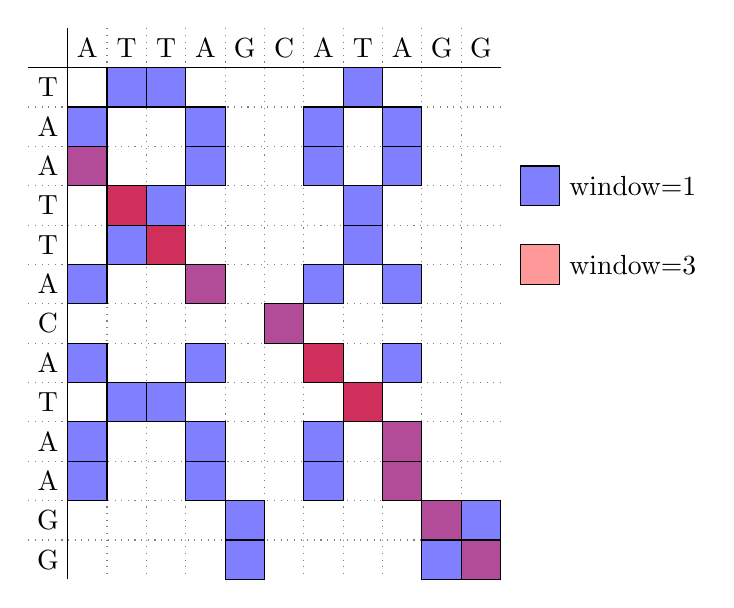
\begin{tikzpicture}[scale=0.5]
      \visible<2->{
\draw [-] (0.5,13.5) -- (12.5,13.5);
\draw [-] (1.5,14.5) -- (1.5,0.5);
	\node at (2,14) {A};
	\draw [-, dotted, opacity=0.5] (2.5,14.5) -- (2.5,0.5);
	\node at (3,14) {T};
	\draw [-, dotted, opacity=0.5] (3.5,14.5) -- (3.5,0.5);
	\node at (4,14) {T};
	\draw [-, dotted, opacity=0.5] (4.5,14.5) -- (4.5,0.5);
	\node at (5,14) {A};
	\draw [-, dotted, opacity=0.5] (5.5,14.5) -- (5.5,0.5);
	\node at (6,14) {G};
	\draw [-, dotted, opacity=0.5] (6.5,14.5) -- (6.5,0.5);
	\node at (7,14) {C};
	\draw [-, dotted, opacity=0.5] (7.5,14.5) -- (7.5,0.5);
	\node at (8,14) {A};
	\draw [-, dotted, opacity=0.5] (8.5,14.5) -- (8.5,0.5);
	\node at (9,14) {T};
	\draw [-, dotted, opacity=0.5] (9.5,14.5) -- (9.5,0.5);
	\node at (10,14) {A};
	\draw [-, dotted, opacity=0.5] (10.5,14.5) -- (10.5,0.5);
	\node at (11,14) {G};
	\draw [-, dotted, opacity=0.5] (11.5,14.5) -- (11.5,0.5);
	\node at (12,14) {G};
	\node at (1,13) {T};
	\draw [-, dotted, opacity=0.5] (0.5,12.5) -- (12.5,12.5);
	\node at (1,12) {A};
	\draw [-, dotted, opacity=0.5] (0.5,11.5) -- (12.5,11.5);
	\node at (1,11) {A};
	\draw [-, dotted, opacity=0.5] (0.5,10.5) -- (12.5,10.5);
	\node at (1,10) {T};
	\draw [-, dotted, opacity=0.5] (0.5,9.5) -- (12.5,9.5);
	\node at (1,9) {T};
	\draw [-, dotted, opacity=0.5] (0.5,8.5) -- (12.5,8.5);
	\node at (1,8) {A};
	\draw [-, dotted, opacity=0.5] (0.5,7.5) -- (12.5,7.5);
	\node at (1,7) {C};
	\draw [-, dotted, opacity=0.5] (0.5,6.5) -- (12.5,6.5);
	\node at (1,6) {A};
	\draw [-, dotted, opacity=0.5] (0.5,5.5) -- (12.5,5.5);
	\node at (1,5) {T};
	\draw [-, dotted, opacity=0.5] (0.5,4.5) -- (12.5,4.5);
	\node at (1,4) {A};
	\draw [-, dotted, opacity=0.5] (0.5,3.5) -- (12.5,3.5);
	\node at (1,3) {A};
	\draw [-, dotted, opacity=0.5] (0.5,2.5) -- (12.5,2.5);
	\node at (1,2) {G};
	\draw [-, dotted, opacity=0.5] (0.5,1.5) -- (12.5,1.5);
	\node at (1,1) {G};
}
\visible<3->{
\draw [fill=blue, fill opacity=0.5] (11 + 2, 13-3) rectangle (11+3,13-2);
\node [right] at (11+3, 13-2.5) { window=1 };
\draw [fill=blue, fill opacity=0.5] (1+1.5,13-0-0.5) rectangle (1+2.5,13-0+0.5);
\draw [fill=blue, fill opacity=0.5] (2+1.5,13-0-0.5) rectangle (2+2.5,13-0+0.5);
\draw [fill=blue, fill opacity=0.5] (7+1.5,13-0-0.5) rectangle (7+2.5,13-0+0.5);
\draw [fill=blue, fill opacity=0.5] (0+1.5,13-1-0.5) rectangle (0+2.5,13-1+0.5);
\draw [fill=blue, fill opacity=0.5] (3+1.5,13-1-0.5) rectangle (3+2.5,13-1+0.5);
\draw [fill=blue, fill opacity=0.5] (6+1.5,13-1-0.5) rectangle (6+2.5,13-1+0.5);
\draw [fill=blue, fill opacity=0.5] (8+1.5,13-1-0.5) rectangle (8+2.5,13-1+0.5);
\draw [fill=blue, fill opacity=0.5] (0+1.5,13-2-0.5) rectangle (0+2.5,13-2+0.5);
\draw [fill=blue, fill opacity=0.5] (3+1.5,13-2-0.5) rectangle (3+2.5,13-2+0.5);
\draw [fill=blue, fill opacity=0.5] (6+1.5,13-2-0.5) rectangle (6+2.5,13-2+0.5);
\draw [fill=blue, fill opacity=0.5] (8+1.5,13-2-0.5) rectangle (8+2.5,13-2+0.5);
\draw [fill=blue, fill opacity=0.5] (1+1.5,13-3-0.5) rectangle (1+2.5,13-3+0.5);
\draw [fill=blue, fill opacity=0.5] (2+1.5,13-3-0.5) rectangle (2+2.5,13-3+0.5);
\draw [fill=blue, fill opacity=0.5] (7+1.5,13-3-0.5) rectangle (7+2.5,13-3+0.5);
\draw [fill=blue, fill opacity=0.5] (1+1.5,13-4-0.5) rectangle (1+2.5,13-4+0.5);
\draw [fill=blue, fill opacity=0.5] (2+1.5,13-4-0.5) rectangle (2+2.5,13-4+0.5);
\draw [fill=blue, fill opacity=0.5] (7+1.5,13-4-0.5) rectangle (7+2.5,13-4+0.5);
\draw [fill=blue, fill opacity=0.5] (0+1.5,13-5-0.5) rectangle (0+2.5,13-5+0.5);
\draw [fill=blue, fill opacity=0.5] (3+1.5,13-5-0.5) rectangle (3+2.5,13-5+0.5);
\draw [fill=blue, fill opacity=0.5] (6+1.5,13-5-0.5) rectangle (6+2.5,13-5+0.5);
\draw [fill=blue, fill opacity=0.5] (8+1.5,13-5-0.5) rectangle (8+2.5,13-5+0.5);
\draw [fill=blue, fill opacity=0.5] (5+1.5,13-6-0.5) rectangle (5+2.5,13-6+0.5);
\draw [fill=blue, fill opacity=0.5] (0+1.5,13-7-0.5) rectangle (0+2.5,13-7+0.5);
\draw [fill=blue, fill opacity=0.5] (3+1.5,13-7-0.5) rectangle (3+2.5,13-7+0.5);
\draw [fill=blue, fill opacity=0.5] (6+1.5,13-7-0.5) rectangle (6+2.5,13-7+0.5);
\draw [fill=blue, fill opacity=0.5] (8+1.5,13-7-0.5) rectangle (8+2.5,13-7+0.5);
\draw [fill=blue, fill opacity=0.5] (1+1.5,13-8-0.5) rectangle (1+2.5,13-8+0.5);
\draw [fill=blue, fill opacity=0.5] (2+1.5,13-8-0.5) rectangle (2+2.5,13-8+0.5);
\draw [fill=blue, fill opacity=0.5] (7+1.5,13-8-0.5) rectangle (7+2.5,13-8+0.5);
\draw [fill=blue, fill opacity=0.5] (0+1.5,13-9-0.5) rectangle (0+2.5,13-9+0.5);
\draw [fill=blue, fill opacity=0.5] (3+1.5,13-9-0.5) rectangle (3+2.5,13-9+0.5);
\draw [fill=blue, fill opacity=0.5] (6+1.5,13-9-0.5) rectangle (6+2.5,13-9+0.5);
\draw [fill=blue, fill opacity=0.5] (8+1.5,13-9-0.5) rectangle (8+2.5,13-9+0.5);
\draw [fill=blue, fill opacity=0.5] (0+1.5,13-10-0.5) rectangle (0+2.5,13-10+0.5);
\draw [fill=blue, fill opacity=0.5] (3+1.5,13-10-0.5) rectangle (3+2.5,13-10+0.5);
\draw [fill=blue, fill opacity=0.5] (6+1.5,13-10-0.5) rectangle (6+2.5,13-10+0.5);
\draw [fill=blue, fill opacity=0.5] (8+1.5,13-10-0.5) rectangle (8+2.5,13-10+0.5);
\draw [fill=blue, fill opacity=0.5] (4+1.5,13-11-0.5) rectangle (4+2.5,13-11+0.5);
\draw [fill=blue, fill opacity=0.5] (9+1.5,13-11-0.5) rectangle (9+2.5,13-11+0.5);
\draw [fill=blue, fill opacity=0.5] (10+1.5,13-11-0.5) rectangle (10+2.5,13-11+0.5);
\draw [fill=blue, fill opacity=0.5] (4+1.5,13-12-0.5) rectangle (4+2.5,13-12+0.5);
\draw [fill=blue, fill opacity=0.5] (9+1.5,13-12-0.5) rectangle (9+2.5,13-12+0.5);
\draw [fill=blue, fill opacity=0.5] (10+1.5,13-12-0.5) rectangle (10+2.5,13-12+0.5);
}
\visible<4->{
\draw [fill=red, fill opacity=0.4] (11 + 2, 13-4) rectangle (11+3,13-5);
\node [right] at (11+3, 13-4.5) { window=3 };
\draw [fill=red, fill opacity=0.4] (0+0+1.5,-0+13-2-0.5) rectangle (0+0+2.5, -0+13-2+0.5);
\draw [fill=red, fill opacity=0.4] (1+0+1.5,-1+13-2-0.5) rectangle (1+0+2.5, -1+13-2+0.5);
\draw [fill=red, fill opacity=0.4] (2+0+1.5,-2+13-2-0.5) rectangle (2+0+2.5, -2+13-2+0.5);
\draw [fill=red, fill opacity=0.4] (0+1+1.5,-0+13-3-0.5) rectangle (0+1+2.5, -0+13-3+0.5);
\draw [fill=red, fill opacity=0.4] (1+1+1.5,-1+13-3-0.5) rectangle (1+1+2.5, -1+13-3+0.5);
\draw [fill=red, fill opacity=0.4] (2+1+1.5,-2+13-3-0.5) rectangle (2+1+2.5, -2+13-3+0.5);
\draw [fill=red, fill opacity=0.4] (0+5+1.5,-0+13-6-0.5) rectangle (0+5+2.5, -0+13-6+0.5);
\draw [fill=red, fill opacity=0.4] (1+5+1.5,-1+13-6-0.5) rectangle (1+5+2.5, -1+13-6+0.5);
\draw [fill=red, fill opacity=0.4] (2+5+1.5,-2+13-6-0.5) rectangle (2+5+2.5, -2+13-6+0.5);
\draw [fill=red, fill opacity=0.4] (0+6+1.5,-0+13-7-0.5) rectangle (0+6+2.5, -0+13-7+0.5);
\draw [fill=red, fill opacity=0.4] (1+6+1.5,-1+13-7-0.5) rectangle (1+6+2.5, -1+13-7+0.5);
\draw [fill=red, fill opacity=0.4] (2+6+1.5,-2+13-7-0.5) rectangle (2+6+2.5, -2+13-7+0.5);
\draw [fill=red, fill opacity=0.4] (0+8+1.5,-0+13-10-0.5) rectangle (0+8+2.5, -0+13-10+0.5);
\draw [fill=red, fill opacity=0.4] (1+8+1.5,-1+13-10-0.5) rectangle (1+8+2.5, -1+13-10+0.5);
\draw [fill=red, fill opacity=0.4] (2+8+1.5,-2+13-10-0.5) rectangle (2+8+2.5, -2+13-10+0.5);
}

    \end{tikzpicture}
  \end{figure}

\end{frame}

\begin{frame}{A dotplot for 4 Mbp region}
%%  \begin{figure}[ht]
  \flushleft
    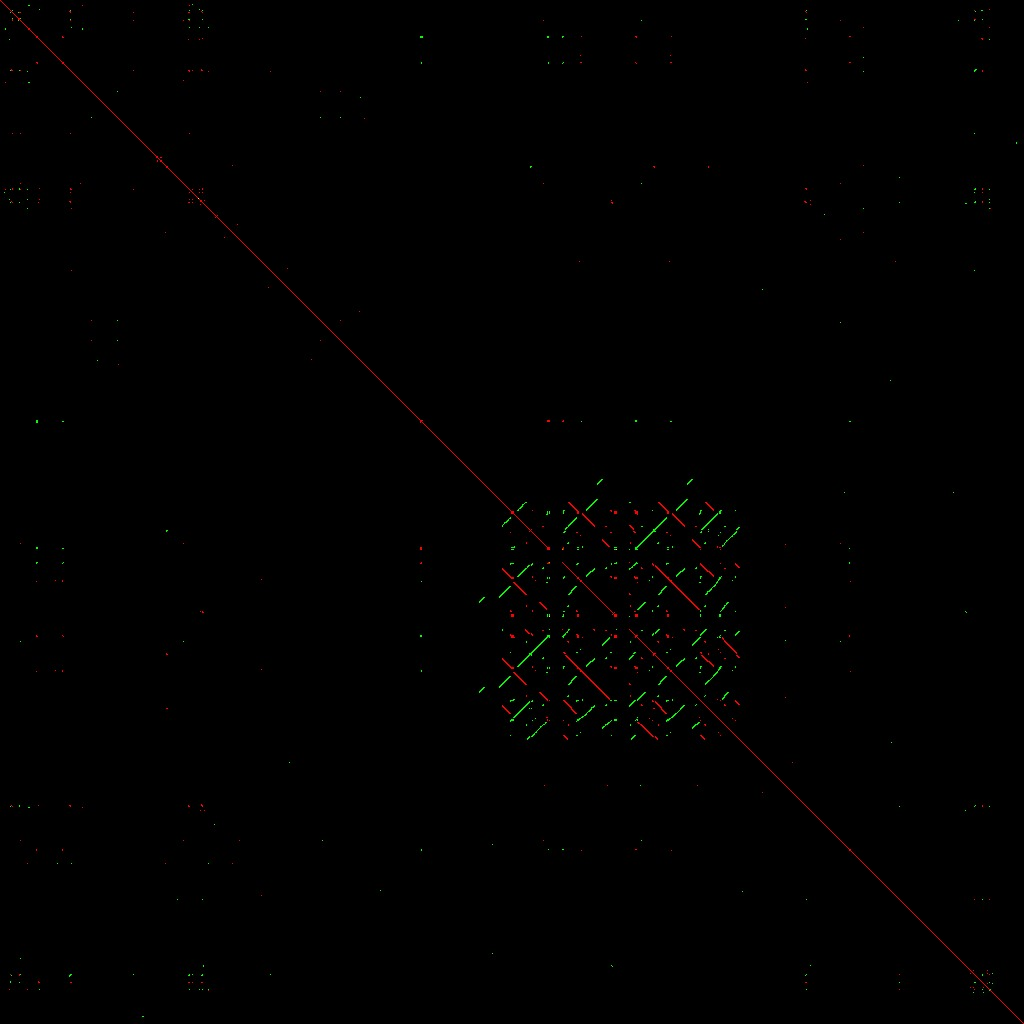
\includegraphics[width=0.8\textwidth]{images/mega_dotter_4_044000001.jpg}
    \hfill
%%  \end{figure}
\end{frame}

\begin{frame}{Dotplot: finding a path}
  \begin{figure}[ht]
    \begin{tikzpicture}[scale=0.35]
      \visible<1->{
\draw [-] (0.5,13.5) -- (12.5,13.5);
\draw [-] (1.5,14.5) -- (1.5,0.5);
	\node at (2,14) {A};
	\draw [-, dotted, opacity=0.5] (2.5,14.5) -- (2.5,0.5);
	\node at (3,14) {T};
	\draw [-, dotted, opacity=0.5] (3.5,14.5) -- (3.5,0.5);
	\node at (4,14) {T};
	\draw [-, dotted, opacity=0.5] (4.5,14.5) -- (4.5,0.5);
	\node at (5,14) {A};
	\draw [-, dotted, opacity=0.5] (5.5,14.5) -- (5.5,0.5);
	\node at (6,14) {G};
	\draw [-, dotted, opacity=0.5] (6.5,14.5) -- (6.5,0.5);
	\node at (7,14) {C};
	\draw [-, dotted, opacity=0.5] (7.5,14.5) -- (7.5,0.5);
	\node at (8,14) {A};
	\draw [-, dotted, opacity=0.5] (8.5,14.5) -- (8.5,0.5);
	\node at (9,14) {T};
	\draw [-, dotted, opacity=0.5] (9.5,14.5) -- (9.5,0.5);
	\node at (10,14) {A};
	\draw [-, dotted, opacity=0.5] (10.5,14.5) -- (10.5,0.5);
	\node at (11,14) {G};
	\draw [-, dotted, opacity=0.5] (11.5,14.5) -- (11.5,0.5);
	\node at (12,14) {G};
	\node at (1,13) {T};
	\draw [-, dotted, opacity=0.5] (0.5,12.5) -- (12.5,12.5);
	\node at (1,12) {A};
	\draw [-, dotted, opacity=0.5] (0.5,11.5) -- (12.5,11.5);
	\node at (1,11) {A};
	\draw [-, dotted, opacity=0.5] (0.5,10.5) -- (12.5,10.5);
	\node at (1,10) {T};
	\draw [-, dotted, opacity=0.5] (0.5,9.5) -- (12.5,9.5);
	\node at (1,9) {T};
	\draw [-, dotted, opacity=0.5] (0.5,8.5) -- (12.5,8.5);
	\node at (1,8) {A};
	\draw [-, dotted, opacity=0.5] (0.5,7.5) -- (12.5,7.5);
	\node at (1,7) {C};
	\draw [-, dotted, opacity=0.5] (0.5,6.5) -- (12.5,6.5);
	\node at (1,6) {A};
	\draw [-, dotted, opacity=0.5] (0.5,5.5) -- (12.5,5.5);
	\node at (1,5) {T};
	\draw [-, dotted, opacity=0.5] (0.5,4.5) -- (12.5,4.5);
	\node at (1,4) {A};
	\draw [-, dotted, opacity=0.5] (0.5,3.5) -- (12.5,3.5);
	\node at (1,3) {A};
	\draw [-, dotted, opacity=0.5] (0.5,2.5) -- (12.5,2.5);
	\node at (1,2) {G};
	\draw [-, dotted, opacity=0.5] (0.5,1.5) -- (12.5,1.5);
	\node at (1,1) {G};
}
\visible<1->{
%%\draw [fill=blue, fill opacity=0.5] (11 + 2, 13-3) rectangle (11+3,13-2);
%%\node [right] at (11+3, 13-2.5) { window=1 };
\draw [fill=blue, fill opacity=0.5] (1+1.5,13-0-0.5) rectangle (1+2.5,13-0+0.5);
\draw [fill=blue, fill opacity=0.5] (2+1.5,13-0-0.5) rectangle (2+2.5,13-0+0.5);
\draw [fill=blue, fill opacity=0.5] (7+1.5,13-0-0.5) rectangle (7+2.5,13-0+0.5);
\draw [fill=blue, fill opacity=0.5] (0+1.5,13-1-0.5) rectangle (0+2.5,13-1+0.5);
\draw [fill=blue, fill opacity=0.5] (3+1.5,13-1-0.5) rectangle (3+2.5,13-1+0.5);
\draw [fill=blue, fill opacity=0.5] (6+1.5,13-1-0.5) rectangle (6+2.5,13-1+0.5);
\draw [fill=blue, fill opacity=0.5] (8+1.5,13-1-0.5) rectangle (8+2.5,13-1+0.5);
\draw [fill=blue, fill opacity=0.5] (0+1.5,13-2-0.5) rectangle (0+2.5,13-2+0.5);
\draw [fill=blue, fill opacity=0.5] (3+1.5,13-2-0.5) rectangle (3+2.5,13-2+0.5);
\draw [fill=blue, fill opacity=0.5] (6+1.5,13-2-0.5) rectangle (6+2.5,13-2+0.5);
\draw [fill=blue, fill opacity=0.5] (8+1.5,13-2-0.5) rectangle (8+2.5,13-2+0.5);
\draw [fill=blue, fill opacity=0.5] (1+1.5,13-3-0.5) rectangle (1+2.5,13-3+0.5);
\draw [fill=blue, fill opacity=0.5] (2+1.5,13-3-0.5) rectangle (2+2.5,13-3+0.5);
\draw [fill=blue, fill opacity=0.5] (7+1.5,13-3-0.5) rectangle (7+2.5,13-3+0.5);
\draw [fill=blue, fill opacity=0.5] (1+1.5,13-4-0.5) rectangle (1+2.5,13-4+0.5);
\draw [fill=blue, fill opacity=0.5] (2+1.5,13-4-0.5) rectangle (2+2.5,13-4+0.5);
\draw [fill=blue, fill opacity=0.5] (7+1.5,13-4-0.5) rectangle (7+2.5,13-4+0.5);
\draw [fill=blue, fill opacity=0.5] (0+1.5,13-5-0.5) rectangle (0+2.5,13-5+0.5);
\draw [fill=blue, fill opacity=0.5] (3+1.5,13-5-0.5) rectangle (3+2.5,13-5+0.5);
\draw [fill=blue, fill opacity=0.5] (6+1.5,13-5-0.5) rectangle (6+2.5,13-5+0.5);
\draw [fill=blue, fill opacity=0.5] (8+1.5,13-5-0.5) rectangle (8+2.5,13-5+0.5);
\draw [fill=blue, fill opacity=0.5] (5+1.5,13-6-0.5) rectangle (5+2.5,13-6+0.5);
\draw [fill=blue, fill opacity=0.5] (0+1.5,13-7-0.5) rectangle (0+2.5,13-7+0.5);
\draw [fill=blue, fill opacity=0.5] (3+1.5,13-7-0.5) rectangle (3+2.5,13-7+0.5);
\draw [fill=blue, fill opacity=0.5] (6+1.5,13-7-0.5) rectangle (6+2.5,13-7+0.5);
\draw [fill=blue, fill opacity=0.5] (8+1.5,13-7-0.5) rectangle (8+2.5,13-7+0.5);
\draw [fill=blue, fill opacity=0.5] (1+1.5,13-8-0.5) rectangle (1+2.5,13-8+0.5);
\draw [fill=blue, fill opacity=0.5] (2+1.5,13-8-0.5) rectangle (2+2.5,13-8+0.5);
\draw [fill=blue, fill opacity=0.5] (7+1.5,13-8-0.5) rectangle (7+2.5,13-8+0.5);
\draw [fill=blue, fill opacity=0.5] (0+1.5,13-9-0.5) rectangle (0+2.5,13-9+0.5);
\draw [fill=blue, fill opacity=0.5] (3+1.5,13-9-0.5) rectangle (3+2.5,13-9+0.5);
\draw [fill=blue, fill opacity=0.5] (6+1.5,13-9-0.5) rectangle (6+2.5,13-9+0.5);
\draw [fill=blue, fill opacity=0.5] (8+1.5,13-9-0.5) rectangle (8+2.5,13-9+0.5);
\draw [fill=blue, fill opacity=0.5] (0+1.5,13-10-0.5) rectangle (0+2.5,13-10+0.5);
\draw [fill=blue, fill opacity=0.5] (3+1.5,13-10-0.5) rectangle (3+2.5,13-10+0.5);
\draw [fill=blue, fill opacity=0.5] (6+1.5,13-10-0.5) rectangle (6+2.5,13-10+0.5);
\draw [fill=blue, fill opacity=0.5] (8+1.5,13-10-0.5) rectangle (8+2.5,13-10+0.5);
\draw [fill=blue, fill opacity=0.5] (4+1.5,13-11-0.5) rectangle (4+2.5,13-11+0.5);
\draw [fill=blue, fill opacity=0.5] (9+1.5,13-11-0.5) rectangle (9+2.5,13-11+0.5);
\draw [fill=blue, fill opacity=0.5] (10+1.5,13-11-0.5) rectangle (10+2.5,13-11+0.5);
\draw [fill=blue, fill opacity=0.5] (4+1.5,13-12-0.5) rectangle (4+2.5,13-12+0.5);
\draw [fill=blue, fill opacity=0.5] (9+1.5,13-12-0.5) rectangle (9+2.5,13-12+0.5);
\draw [fill=blue, fill opacity=0.5] (10+1.5,13-12-0.5) rectangle (10+2.5,13-12+0.5);
}
\visible<1->{
%%\draw [fill=red, fill opacity=0.4] (11 + 2, 13-4) rectangle (11+3,13-5);
%%\node [right] at (11+3, 13-4.5) { window=3 };
\draw [fill=red, fill opacity=0.4] (0+0+1.5,-0+13-2-0.5) rectangle (0+0+2.5, -0+13-2+0.5);
\draw [fill=red, fill opacity=0.4] (1+0+1.5,-1+13-2-0.5) rectangle (1+0+2.5, -1+13-2+0.5);
\draw [fill=red, fill opacity=0.4] (2+0+1.5,-2+13-2-0.5) rectangle (2+0+2.5, -2+13-2+0.5);
\draw [fill=red, fill opacity=0.4] (0+1+1.5,-0+13-3-0.5) rectangle (0+1+2.5, -0+13-3+0.5);
\draw [fill=red, fill opacity=0.4] (1+1+1.5,-1+13-3-0.5) rectangle (1+1+2.5, -1+13-3+0.5);
\draw [fill=red, fill opacity=0.4] (2+1+1.5,-2+13-3-0.5) rectangle (2+1+2.5, -2+13-3+0.5);
\draw [fill=red, fill opacity=0.4] (0+5+1.5,-0+13-6-0.5) rectangle (0+5+2.5, -0+13-6+0.5);
\draw [fill=red, fill opacity=0.4] (1+5+1.5,-1+13-6-0.5) rectangle (1+5+2.5, -1+13-6+0.5);
\draw [fill=red, fill opacity=0.4] (2+5+1.5,-2+13-6-0.5) rectangle (2+5+2.5, -2+13-6+0.5);
\draw [fill=red, fill opacity=0.4] (0+6+1.5,-0+13-7-0.5) rectangle (0+6+2.5, -0+13-7+0.5);
\draw [fill=red, fill opacity=0.4] (1+6+1.5,-1+13-7-0.5) rectangle (1+6+2.5, -1+13-7+0.5);
\draw [fill=red, fill opacity=0.4] (2+6+1.5,-2+13-7-0.5) rectangle (2+6+2.5, -2+13-7+0.5);
\draw [fill=red, fill opacity=0.4] (0+8+1.5,-0+13-10-0.5) rectangle (0+8+2.5, -0+13-10+0.5);
\draw [fill=red, fill opacity=0.4] (1+8+1.5,-1+13-10-0.5) rectangle (1+8+2.5, -1+13-10+0.5);
\draw [fill=red, fill opacity=0.4] (2+8+1.5,-2+13-10-0.5) rectangle (2+8+2.5, -2+13-10+0.5);
}

      \def\s{0.8}
      \visible<2->{
        \def\x{2}
        \def\y{13}
        \draw [->] (\x,\y) -- (\x+\s,\y);
        \draw [->] (\x,\y) -- (\x,\y-\s);
        \draw [->] (\x,\y) -- (\x+\s,\y-\s);
      }
      \visible<3->{
        \def\x{3}
        \def\y{13}
        \draw [->] (\x,\y) -- (\x+\s,\y);
        \draw [->] (\x,\y) -- (\x,\y-\s);
        \draw [->] (\x,\y) -- (\x+\s,\y-\s);
      }
      \visible<4->{
        \def\x{2}
        \def\y{12}
        \draw [->] (\x,\y) -- (\x+\s,\y);
        \draw [->] (\x,\y) -- (\x,\y-\s);
        \draw [->] (\x,\y) -- (\x+\s,\y-\s);
      }
      \visible<5->{
        \def\x{3}
        \def\y{12}
        \draw [->] (\x,\y) -- (\x+\s,\y);
        \draw [->] (\x,\y) -- (\x,\y-\s);
        \draw [->] (\x,\y) -- (\x+\s,\y-\s);
      }
      \visible<6->{
        \node [below right, align=left] at (0,0) {No Equation??\\$\rightarrow$
          write a program};
      }
      \visible<7->{
        \node[inner sep=0pt, below right] at (15,17) {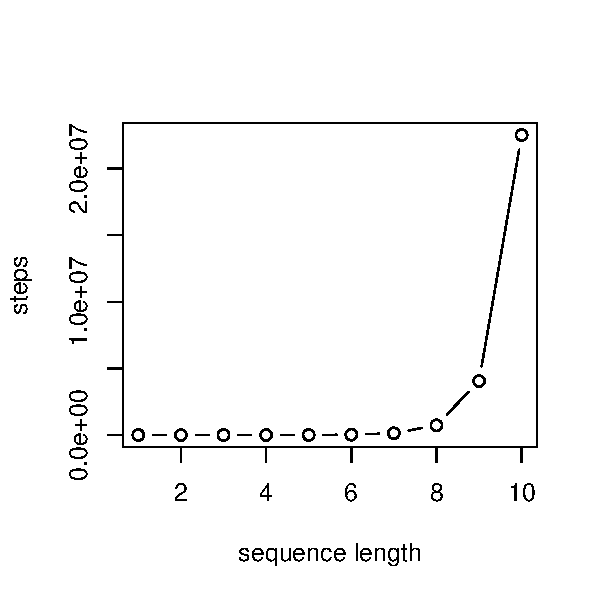
\includegraphics[width=.4\textwidth]{R/step_counts.pdf}};
        \node[inner sep=0pt, below right] at (15,7) {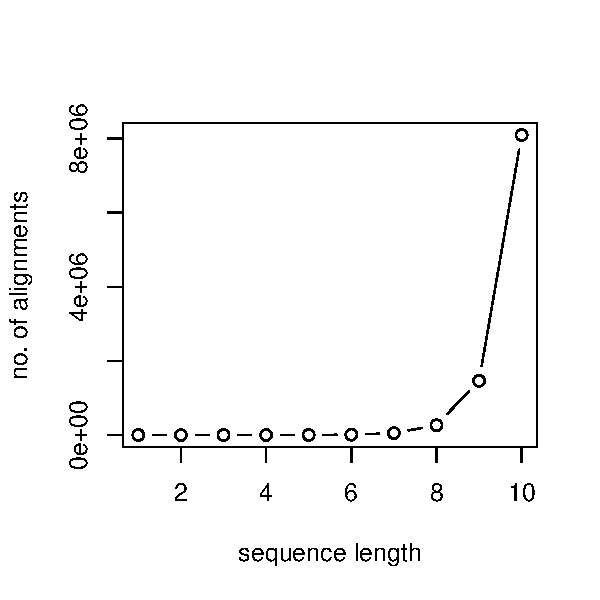
\includegraphics[width=.4\textwidth]{R/alignment_counts.pdf}};
      }
    \end{tikzpicture}
  \end{figure}
  
\end{frame}


\begin{frame}{Optimal alignments}
  Dotplot gives a visualisation, but does not lead directly to
  an optimal alignment. Two different kinds of optimal alignment.
  \begin{description}
  \item[Global] Aligns two complete sequences to each other. Can
    be achieved by the \textcolor{navy}{\emph{Needleman-Wunsch}} algorithm.
  \item[Local] Finds the maximally scoring subalignment present
    between two sequences. Can be obtained by the \textcolor{navy}{\emph{Smith-Waterman}}
    algorithm.
  \end{description}
  \pause
  These are examples of \textcolor{navy}{\emph{dynamic programming}} methods.

  \textcolor{navy}{\emph{Optimal}} : the highest scoring alignment for a given scoring scheme.

  There is \emph{no best alignment} for two sequences. \emph{Best} depends on
  the biological question asked, and the specific method (local/global) and
  scoring method and parameters have to be selected for the question.
\end{frame}

\begin{frame}{Needleman-Wunsch: global alignment}
  \begin{figure}[ht]
    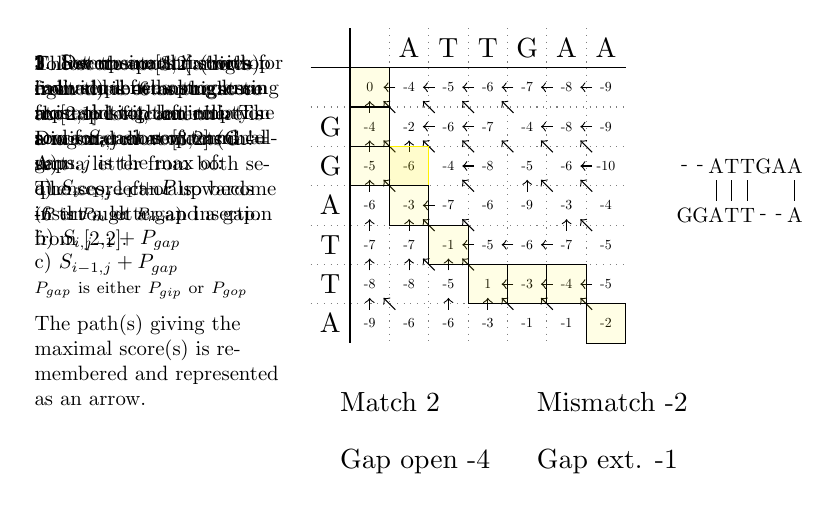
\begin{tikzpicture}[scale=0.5]
      \node [right] at (1,-1) {Match 2};
\node [right] at (6,-1) {Mismatch -2};
\node [right] at (1,-2.5) {Gap open -4};
\node [right] at (6,-2.5) {Gap ext. -1};

\draw [-] (0.5,7.5) -- (8.5,7.5);
\draw [-] (1.5,8.5) -- (1.5,0.5);
\draw [-, dotted, opacity=0.5] (0.5,6.5) -- (8.5,6.5);
\draw [-, dotted, opacity=0.5] (2.5,8.5) -- (2.5,0.5);
	\node at (3,8) {A};
	\draw [-, dotted, opacity=0.5] (3.5,8.5) -- (3.5,0.5);
	\node at (4,8) {T};
	\draw [-, dotted, opacity=0.5] (4.5,8.5) -- (4.5,0.5);
	\node at (5,8) {T};
	\draw [-, dotted, opacity=0.5] (5.5,8.5) -- (5.5,0.5);
	\node at (6,8) {G};
	\draw [-, dotted, opacity=0.5] (6.5,8.5) -- (6.5,0.5);
	\node at (7,8) {A};
	\draw [-, dotted, opacity=0.5] (7.5,8.5) -- (7.5,0.5);
	\node at (8,8) {A};
	\node at (1,6) {G};
	\draw [-, dotted, opacity=0.5] (0.5,5.5) -- (8.5,5.5);
	\node at (1,5) {G};
	\draw [-, dotted, opacity=0.5] (0.5,4.5) -- (8.5,4.5);
	\node at (1,4) {A};
	\draw [-, dotted, opacity=0.5] (0.5,3.5) -- (8.5,3.5);
	\node at (1,3) {T};
	\draw [-, dotted, opacity=0.5] (0.5,2.5) -- (8.5,2.5);
	\node at (1,2) {T};
	\draw [-, dotted, opacity=0.5] (0.5,1.5) -- (8.5,1.5);
	\node at (1,1) {A};



	\node [below left, align=left, scale=0.75, text width=12em] 
	at (0,8) {1. Set up a matrix with each sequence 
	along an axis and with an empty row for each sequence.};



	\node[scale=0.5] at (2,7) {0};
	\node[scale=0.5] at (3,7) {-4};
	\draw [->] (2.65, 6+1) -- (2.35, 6+1);
	\node[scale=0.5] at(4,7) {-5};
	\draw [->] (3.65,6+1) -- (3.35,6+1);
	\node[scale=0.5] at(5,7) {-6};
	\draw [->] (4.65,6+1) -- (4.35,6+1);
	\node[scale=0.5] at(6,7) {-7};
	\draw [->] (5.65,6+1) -- (5.35,6+1);
	\node[scale=0.5] at(7,7) {-8};
	\draw [->] (6.65,6+1) -- (6.35,6+1);
	\node[scale=0.5] at(8,7) {-9};
	\draw [->] (7.65,6+1) -- (7.35,6+1);
	\node[scale=0.5] at (2,6) {-4};
	\draw [->] (2,6 + 0.35) -- (2, 6 + 0.65);
	\node[scale=0.5] at(2,5) {-5};
	\draw [->] (2,6-1 + 0.35) -- (2, 6-1 + 0.65);
	\node[scale=0.5] at(2,4) {-6};
	\draw [->] (2,6-2 + 0.35) -- (2, 6-2 + 0.65);
	\node[scale=0.5] at(2,3) {-7};
	\draw [->] (2,6-3 + 0.35) -- (2, 6-3 + 0.65);
	\node[scale=0.5] at(2,2) {-8};
	\draw [->] (2,6-4 + 0.35) -- (2, 6-4 + 0.65);
	\node[scale=0.5] at(2,1) {-9};
	\draw [->] (2,6-5 + 0.35) -- (2, 6-5 + 0.65);



	\node [below left, align=left, scale=0.75, text width=12em] 
	at (0,8) {2. Insert scores in the top row and left-most column representing
	the initiation and extension of terminal gaps.};



	\node [scale=0.5] at (3,6) {-2};
	\draw [->] (2.65,6.35) -- (2.35,6.65);
	\node [scale=0.5] at (4,6) {-6};
	\draw [->] (3.65,6.35) -- (3.35,6.65);
	\draw [->] (3.65,6) -- (3.35,6);
	\node [scale=0.5] at (5,6) {-7};
	\draw [->] (4.65,6.35) -- (4.35,6.65);
	\draw [->] (4.65,6) -- (4.35,6);
	\node [scale=0.5] at (6,6) {-4};
	\draw [->] (5.65,6.35) -- (5.35,6.65);
	\node [scale=0.5] at (7,6) {-8};
	\draw [->] (6.65,6) -- (6.35,6);
	\node [scale=0.5] at (8,6) {-9};
	\draw [->] (7.65,6) -- (7.35,6);



	\node [below left, align=left, scale=0.75, text width=12em] 
	at (0,8) {3. Determine the scores for individual cells progressing from
	the top left cell. The score $S_{i,j}$ at row $i$ and column $j$ is the max of:\\
	a) $S_{i-1,j-1} + P$\\
	{\footnotesize($P$ is $P_m$ or $P_{mm}$).
	}\\
	b) $S_{i,j-1} + P_{gap}$\\
	c) $S_{i-1,j} + P_{gap}$\\
	{\footnotesize $P_{gap}$ is either $P_{gip}$ or $P_{gop}$}\\
	\vspace{0.2cm}
	The path(s) giving the maximal score(s) is remembered and represented as
	an arrow.
	};




	\node [scale=0.5] at (3,5) {-6};
	\draw [->] (2.65,5.35) -- (2.35,5.65);
	\draw [->] (3,5.35) -- (3,5.65);
	\node [scale=0.5] at (4,5) {-4};
	\draw [->] (3.65,5.35) -- (3.35,5.65);
	\node [scale=0.5] at (5,5) {-8};
	\draw [->] (4.65,5.35) -- (4.35,5.65);
	\draw [->] (4.65,5) -- (4.35,5);
	\node [scale=0.5] at (6,5) {-5};
	\draw [->] (5.65,5.35) -- (5.35,5.65);
	\node [scale=0.5] at (7,5) {-6};
	\draw [->] (6.65,5.35) -- (6.35,5.65);
	\node [scale=0.5] at (8,5) {-10};
	\draw [->] (7.65,5.35) -- (7.35,5.65);
	\draw [->] (7.65,5) -- (7.35,5);



	\draw [fill, yellow, fill opacity=0.2] (2.5,4.5) rectangle (3.5,5.5);
	\node [below left, align=left, scale=0.75, text width=12em] 
	at (0,8) {
	The score at [3,2] (highlighted) is -6 as the score at [2,1] is -4, and there is a
	mismatch at [3,2] (G != A). 

	The score can also become -6 through a gap
	insertion from [2,2].
	};




	\node [scale=0.5] at (3,4) {-3};
	\draw [->] (2.65,4.35) -- (2.35,4.65);
	\node [scale=0.5] at (4,4) {-7};
	\draw [->] (3.65,4) -- (3.35,4);
	\node [scale=0.5] at (5,4) {-6};
	\draw [->] (4.65,4.35) -- (4.35,4.65);
	\node [scale=0.5] at (6,4) {-9};
	\draw [->] (6,4.35) -- (6,4.65);
	\node [scale=0.5] at (7,4) {-3};
	\draw [->] (6.65,4.35) -- (6.35,4.65);
	\node [scale=0.5] at (8,4) {-4};
	\draw [->] (7.65,4.35) -- (7.35,4.65);


	\node [scale=0.5] at (3,3) {-7};
	\draw [->] (3,3.35) -- (3,3.65);
	\node [scale=0.5] at (4,3) {-1};
	\draw [->] (3.65,3.35) -- (3.35,3.65);
	\node [scale=0.5] at (5,3) {-5};
	\draw [->] (4.65,3.35) -- (4.35,3.65);
	\draw [->] (4.65,3) -- (4.35,3);
	\node [scale=0.5] at (6,3) {-6};
	\draw [->] (5.65,3) -- (5.35,3);
	\node [scale=0.5] at (7,3) {-7};
	\draw [->] (6.65,3) -- (6.35,3);
	\draw [->] (7,3.35) -- (7,3.65);
	\node [scale=0.5] at (8,3) {-5};
	\draw [->] (7.65,3.35) -- (7.35,3.65);


	\node [scale=0.5] at (3,2) {-8};
	\draw [->] (3,2.35) -- (3,2.65);
	\node [scale=0.5] at (4,2) {-5};
	\draw [->] (3.65,2.35) -- (3.35,2.65);
	\draw [->] (4,2.35) -- (4,2.65);
	\node [scale=0.5] at (5,2) {1};
	\draw [->] (4.65,2.35) -- (4.35,2.65);
	\node [scale=0.5] at (6,2) {-3};
	\draw [->] (5.65,2) -- (5.35,2);
	\node [scale=0.5] at (7,2) {-4};
	\draw [->] (6.65,2) -- (6.35,2);
	\node [scale=0.5] at (8,2) {-5};
	\draw [->] (7.65,2) -- (7.35,2);


	\node [scale=0.5] at (3,1) {-6};
	\draw [->] (2.65,1.35) -- (2.35,1.65);
	\node [scale=0.5] at (4,1) {-6};
	\draw [->] (4,1.35) -- (4,1.65);
	\node [scale=0.5] at (5,1) {-3};
	\draw [->] (5,1.35) -- (5,1.65);
	\node [scale=0.5] at (6,1) {-1};
	\draw [->] (5.65,1.35) -- (5.35,1.65);
	\node [scale=0.5] at (7,1) {-1};
	\draw [->] (6.65,1.35) -- (6.35,1.65);
	\node [scale=0.5] at (8,1) {-2};
	\draw [->] (7.65,1.35) -- (7.35,1.65);

\draw [fill=yellow, fill opacity=0.1] (7.5,0.5) rectangle (8.5,1.5);


\draw [fill=yellow, fill opacity=0.1] (6.5,1.5) rectangle (7.5,2.5);


\draw [fill=yellow, fill opacity=0.1] (5.5,1.5) rectangle (6.5,2.5);


\draw [fill=yellow, fill opacity=0.1] (4.5,1.5) rectangle (5.5,2.5);


\draw [fill=yellow, fill opacity=0.1] (3.5,2.5) rectangle (4.5,3.5);


\draw [fill=yellow, fill opacity=0.1] (2.5,3.5) rectangle (3.5,4.5);


\draw [fill=yellow, fill opacity=0.1] (1.5,4.5) rectangle (2.5,5.5);


\draw [fill=yellow, fill opacity=0.1] (1.5,5.5) rectangle (2.5,6.5);


\draw [fill=yellow, fill opacity=0.1] (1.5,6.5) rectangle (2.5,7.5);



	\node [below left, align=left, scale=0.75, text width=12em] 
	at (0,8) {
	Follow the path (arrows) from the bottom right to
	the top left corner.

	Diagonal movements insert a letter from both sequences,
	left or upwards insert a letter and a gap.
	};



\node [scale=0.75] (s1) at (10 + 0/2.5, 5) {-};
\node [scale=0.75] (s2) at (10 + 0/2.5, 5-1.25) {G};
\node [scale=0.75] (s1) at (10 + 1/2.5, 5) {-};
\node [scale=0.75] (s2) at (10 + 1/2.5, 5-1.25) {G};
\node [scale=0.75] (s1) at (10 + 2/2.5, 5) {A};
\node [scale=0.75] (s2) at (10 + 2/2.5, 5-1.25) {A};
\draw [-] (s1) -- (s2);
\node [scale=0.75] (s1) at (10 + 3/2.5, 5) {T};
\node [scale=0.75] (s2) at (10 + 3/2.5, 5-1.25) {T};
\draw [-] (s1) -- (s2);
\node [scale=0.75] (s1) at (10 + 4/2.5, 5) {T};
\node [scale=0.75] (s2) at (10 + 4/2.5, 5-1.25) {T};
\draw [-] (s1) -- (s2);
\node [scale=0.75] (s1) at (10 + 5/2.5, 5) {G};
\node [scale=0.75] (s2) at (10 + 5/2.5, 5-1.25) {-};
\node [scale=0.75] (s1) at (10 + 6/2.5, 5) {A};
\node [scale=0.75] (s2) at (10 + 6/2.5, 5-1.25) {-};
\node [scale=0.75] (s1) at (10 + 7/2.5, 5) {A};
\node [scale=0.75] (s2) at (10 + 7/2.5, 5-1.25) {A};
\draw [-] (s1) -- (s2);


    \end{tikzpicture}
  \end{figure}

\end{frame}

\begin{frame}{Needleman-Wunsch (2): a bigger example}
  \begin{figure}[ht]
    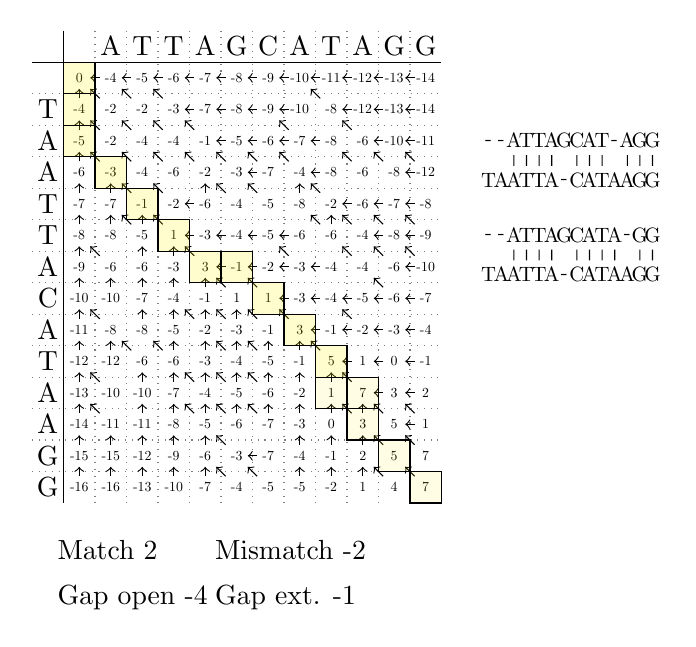
\begin{tikzpicture}[scale=0.4]
      \node [right] at (1,-1) {Match 2};
\node [right] at (6,-1) {Mismatch -2};
\node [right] at (1,-2.5) {Gap open -4};
\node [right] at (6,-2.5) {Gap ext. -1};
\visible<2->{
\draw [-] (0.5,14.5) -- (13.5,14.5);
\draw [-] (1.5,15.5) -- (1.5,0.5);
\draw [-, dotted, opacity=0.5] (0.5,13.5) -- (13.5,13.5);
\draw [-, dotted, opacity=0.5] (2.5,15.5) -- (2.5,0.5);
	\node at (3,15) {A};
	\draw [-, dotted, opacity=0.5] (3.5,15.5) -- (3.5,0.5);
	\node at (4,15) {T};
	\draw [-, dotted, opacity=0.5] (4.5,15.5) -- (4.5,0.5);
	\node at (5,15) {T};
	\draw [-, dotted, opacity=0.5] (5.5,15.5) -- (5.5,0.5);
	\node at (6,15) {A};
	\draw [-, dotted, opacity=0.5] (6.5,15.5) -- (6.5,0.5);
	\node at (7,15) {G};
	\draw [-, dotted, opacity=0.5] (7.5,15.5) -- (7.5,0.5);
	\node at (8,15) {C};
	\draw [-, dotted, opacity=0.5] (8.5,15.5) -- (8.5,0.5);
	\node at (9,15) {A};
	\draw [-, dotted, opacity=0.5] (9.5,15.5) -- (9.5,0.5);
	\node at (10,15) {T};
	\draw [-, dotted, opacity=0.5] (10.5,15.5) -- (10.5,0.5);
	\node at (11,15) {A};
	\draw [-, dotted, opacity=0.5] (11.5,15.5) -- (11.5,0.5);
	\node at (12,15) {G};
	\draw [-, dotted, opacity=0.5] (12.5,15.5) -- (12.5,0.5);
	\node at (13,15) {G};
	\node at (1,13) {T};
	\draw [-, dotted, opacity=0.5] (0.5,12.5) -- (13.5,12.5);
	\node at (1,12) {A};
	\draw [-, dotted, opacity=0.5] (0.5,11.5) -- (13.5,11.5);
	\node at (1,11) {A};
	\draw [-, dotted, opacity=0.5] (0.5,10.5) -- (13.5,10.5);
	\node at (1,10) {T};
	\draw [-, dotted, opacity=0.5] (0.5,9.5) -- (13.5,9.5);
	\node at (1,9) {T};
	\draw [-, dotted, opacity=0.5] (0.5,8.5) -- (13.5,8.5);
	\node at (1,8) {A};
	\draw [-, dotted, opacity=0.5] (0.5,7.5) -- (13.5,7.5);
	\node at (1,7) {C};
	\draw [-, dotted, opacity=0.5] (0.5,6.5) -- (13.5,6.5);
	\node at (1,6) {A};
	\draw [-, dotted, opacity=0.5] (0.5,5.5) -- (13.5,5.5);
	\node at (1,5) {T};
	\draw [-, dotted, opacity=0.5] (0.5,4.5) -- (13.5,4.5);
	\node at (1,4) {A};
	\draw [-, dotted, opacity=0.5] (0.5,3.5) -- (13.5,3.5);
	\node at (1,3) {A};
	\draw [-, dotted, opacity=0.5] (0.5,2.5) -- (13.5,2.5);
	\node at (1,2) {G};
	\draw [-, dotted, opacity=0.5] (0.5,1.5) -- (13.5,1.5);
	\node at (1,1) {G};
}
\visible<3->{
	\node[scale=0.5] at (2,14) {0};
	\node[scale=0.5] at (3,14) {-4};
	\draw [->] (2.65, 13+1) -- (2.35, 13+1);
	\node[scale=0.5] at(4,14) {-5};
	\draw [->] (3.65,13+1) -- (3.35,13+1);
	\node[scale=0.5] at(5,14) {-6};
	\draw [->] (4.65,13+1) -- (4.35,13+1);
	\node[scale=0.5] at(6,14) {-7};
	\draw [->] (5.65,13+1) -- (5.35,13+1);
	\node[scale=0.5] at(7,14) {-8};
	\draw [->] (6.65,13+1) -- (6.35,13+1);
	\node[scale=0.5] at(8,14) {-9};
	\draw [->] (7.65,13+1) -- (7.35,13+1);
	\node[scale=0.5] at(9,14) {-10};
	\draw [->] (8.65,13+1) -- (8.35,13+1);
	\node[scale=0.5] at(10,14) {-11};
	\draw [->] (9.65,13+1) -- (9.35,13+1);
	\node[scale=0.5] at(11,14) {-12};
	\draw [->] (10.65,13+1) -- (10.35,13+1);
	\node[scale=0.5] at(12,14) {-13};
	\draw [->] (11.65,13+1) -- (11.35,13+1);
	\node[scale=0.5] at(13,14) {-14};
	\draw [->] (12.65,13+1) -- (12.35,13+1);
	\node[scale=0.5] at (2,13) {-4};
	\draw [->] (2,13 + 0.35) -- (2, 13 + 0.65);
	\node[scale=0.5] at(2,12) {-5};
	\draw [->] (2,13-1 + 0.35) -- (2, 13-1 + 0.65);
	\node[scale=0.5] at(2,11) {-6};
	\draw [->] (2,13-2 + 0.35) -- (2, 13-2 + 0.65);
	\node[scale=0.5] at(2,10) {-7};
	\draw [->] (2,13-3 + 0.35) -- (2, 13-3 + 0.65);
	\node[scale=0.5] at(2,9) {-8};
	\draw [->] (2,13-4 + 0.35) -- (2, 13-4 + 0.65);
	\node[scale=0.5] at(2,8) {-9};
	\draw [->] (2,13-5 + 0.35) -- (2, 13-5 + 0.65);
	\node[scale=0.5] at(2,7) {-10};
	\draw [->] (2,13-6 + 0.35) -- (2, 13-6 + 0.65);
	\node[scale=0.5] at(2,6) {-11};
	\draw [->] (2,13-7 + 0.35) -- (2, 13-7 + 0.65);
	\node[scale=0.5] at(2,5) {-12};
	\draw [->] (2,13-8 + 0.35) -- (2, 13-8 + 0.65);
	\node[scale=0.5] at(2,4) {-13};
	\draw [->] (2,13-9 + 0.35) -- (2, 13-9 + 0.65);
	\node[scale=0.5] at(2,3) {-14};
	\draw [->] (2,13-10 + 0.35) -- (2, 13-10 + 0.65);
	\node[scale=0.5] at(2,2) {-15};
	\draw [->] (2,13-11 + 0.35) -- (2, 13-11 + 0.65);
	\node[scale=0.5] at(2,1) {-16};
	\draw [->] (2,13-12 + 0.35) -- (2, 13-12 + 0.65);
}
\visible<4->{
	\node [scale=0.5] at (3,13) {-2};
	\draw [->] (2.65,13.35) -- (2.35,13.65);
	\node [scale=0.5] at (4,13) {-2};
	\draw [->] (3.65,13.35) -- (3.35,13.65);
	\node [scale=0.5] at (5,13) {-3};
	\draw [->] (4.65,13.35) -- (4.35,13.65);
	\node [scale=0.5] at (6,13) {-7};
	\draw [->] (5.65,13) -- (5.35,13);
	\node [scale=0.5] at (7,13) {-8};
	\draw [->] (6.65,13) -- (6.35,13);
	\node [scale=0.5] at (8,13) {-9};
	\draw [->] (7.65,13) -- (7.35,13);
	\node [scale=0.5] at (9,13) {-10};
	\draw [->] (8.65,13) -- (8.35,13);
	\node [scale=0.5] at (10,13) {-8};
	\draw [->] (9.65,13.35) -- (9.35,13.65);
	\node [scale=0.5] at (11,13) {-12};
	\draw [->] (10.65,13) -- (10.35,13);
	\node [scale=0.5] at (12,13) {-13};
	\draw [->] (11.65,13) -- (11.35,13);
	\node [scale=0.5] at (13,13) {-14};
	\draw [->] (12.65,13) -- (12.35,13);
}
\visible<5->{
	\node [scale=0.5] at (3,12) {-2};
	\draw [->] (2.65,12.35) -- (2.35,12.65);
	\node [scale=0.5] at (4,12) {-4};
	\draw [->] (3.65,12.35) -- (3.35,12.65);
	\node [scale=0.5] at (5,12) {-4};
	\draw [->] (4.65,12.35) -- (4.35,12.65);
	\node [scale=0.5] at (6,12) {-1};
	\draw [->] (5.65,12.35) -- (5.35,12.65);
	\node [scale=0.5] at (7,12) {-5};
	\draw [->] (6.65,12) -- (6.35,12);
	\node [scale=0.5] at (8,12) {-6};
	\draw [->] (7.65,12) -- (7.35,12);
	\node [scale=0.5] at (9,12) {-7};
	\draw [->] (8.65,12.35) -- (8.35,12.65);
	\draw [->] (8.65,12) -- (8.35,12);
	\node [scale=0.5] at (10,12) {-8};
	\draw [->] (9.65,12) -- (9.35,12);
	\node [scale=0.5] at (11,12) {-6};
	\draw [->] (10.65,12.35) -- (10.35,12.65);
	\node [scale=0.5] at (12,12) {-10};
	\draw [->] (11.65,12) -- (11.35,12);
	\node [scale=0.5] at (13,12) {-11};
	\draw [->] (12.65,12) -- (12.35,12);
}
\visible<6->{
	\node [scale=0.5] at (3,11) {-3};
	\draw [->] (2.65,11.35) -- (2.35,11.65);
	\node [scale=0.5] at (4,11) {-4};
	\draw [->] (3.65,11.35) -- (3.35,11.65);
	\node [scale=0.5] at (5,11) {-6};
	\draw [->] (4.65,11.35) -- (4.35,11.65);
	\node [scale=0.5] at (6,11) {-2};
	\draw [->] (5.65,11.35) -- (5.35,11.65);
	\node [scale=0.5] at (7,11) {-3};
	\draw [->] (6.65,11.35) -- (6.35,11.65);
	\node [scale=0.5] at (8,11) {-7};
	\draw [->] (7.65,11.35) -- (7.35,11.65);
	\draw [->] (7.65,11) -- (7.35,11);
	\node [scale=0.5] at (9,11) {-4};
	\draw [->] (8.65,11.35) -- (8.35,11.65);
	\node [scale=0.5] at (10,11) {-8};
	\draw [->] (9.65,11) -- (9.35,11);
	\node [scale=0.5] at (11,11) {-6};
	\draw [->] (10.65,11.35) -- (10.35,11.65);
	\node [scale=0.5] at (12,11) {-8};
	\draw [->] (11.65,11.35) -- (11.35,11.65);
	\node [scale=0.5] at (13,11) {-12};
	\draw [->] (12.65,11.35) -- (12.35,11.65);
	\draw [->] (12.65,11) -- (12.35,11);
}
\visible<7->{
	\node [scale=0.5] at (3,10) {-7};
	\draw [->] (3,10.35) -- (3,10.65);
	\node [scale=0.5] at (4,10) {-1};
	\draw [->] (3.65,10.35) -- (3.35,10.65);
	\node [scale=0.5] at (5,10) {-2};
	\draw [->] (4.65,10.35) -- (4.35,10.65);
	\node [scale=0.5] at (6,10) {-6};
	\draw [->] (5.65,10) -- (5.35,10);
	\draw [->] (6,10.35) -- (6,10.65);
	\node [scale=0.5] at (7,10) {-4};
	\draw [->] (6.65,10.35) -- (6.35,10.65);
	\node [scale=0.5] at (8,10) {-5};
	\draw [->] (7.65,10.35) -- (7.35,10.65);
	\node [scale=0.5] at (9,10) {-8};
	\draw [->] (9,10.35) -- (9,10.65);
	\node [scale=0.5] at (10,10) {-2};
	\draw [->] (9.65,10.35) -- (9.35,10.65);
	\node [scale=0.5] at (11,10) {-6};
	\draw [->] (10.65,10) -- (10.35,10);
	\node [scale=0.5] at (12,10) {-7};
	\draw [->] (11.65,10) -- (11.35,10);
	\node [scale=0.5] at (13,10) {-8};
	\draw [->] (12.65,10) -- (12.35,10);
}
\visible<8->{
	\node [scale=0.5] at (3,9) {-8};
	\draw [->] (3,9.35) -- (3,9.65);
	\node [scale=0.5] at (4,9) {-5};
	\draw [->] (3.65,9.35) -- (3.35,9.65);
	\draw [->] (4,9.35) -- (4,9.65);
	\node [scale=0.5] at (5,9) {1};
	\draw [->] (4.65,9.35) -- (4.35,9.65);
	\node [scale=0.5] at (6,9) {-3};
	\draw [->] (5.65,9) -- (5.35,9);
	\node [scale=0.5] at (7,9) {-4};
	\draw [->] (6.65,9) -- (6.35,9);
	\node [scale=0.5] at (8,9) {-5};
	\draw [->] (7.65,9) -- (7.35,9);
	\node [scale=0.5] at (9,9) {-6};
	\draw [->] (8.65,9) -- (8.35,9);
	\node [scale=0.5] at (10,9) {-6};
	\draw [->] (9.65,9.35) -- (9.35,9.65);
	\draw [->] (10,9.35) -- (10,9.65);
	\node [scale=0.5] at (11,9) {-4};
	\draw [->] (10.65,9.35) -- (10.35,9.65);
	\node [scale=0.5] at (12,9) {-8};
	\draw [->] (11.65,9.35) -- (11.35,9.65);
	\draw [->] (11.65,9) -- (11.35,9);
	\node [scale=0.5] at (13,9) {-9};
	\draw [->] (12.65,9.35) -- (12.35,9.65);
	\draw [->] (12.65,9) -- (12.35,9);
}
\visible<9->{
	\node [scale=0.5] at (3,8) {-6};
	\draw [->] (2.65,8.35) -- (2.35,8.65);
	\node [scale=0.5] at (4,8) {-6};
	\draw [->] (4,8.35) -- (4,8.65);
	\node [scale=0.5] at (5,8) {-3};
	\draw [->] (5,8.35) -- (5,8.65);
	\node [scale=0.5] at (6,8) {3};
	\draw [->] (5.65,8.35) -- (5.35,8.65);
	\node [scale=0.5] at (7,8) {-1};
	\draw [->] (6.65,8) -- (6.35,8);
	\node [scale=0.5] at (8,8) {-2};
	\draw [->] (7.65,8) -- (7.35,8);
	\node [scale=0.5] at (9,8) {-3};
	\draw [->] (8.65,8.35) -- (8.35,8.65);
	\draw [->] (8.65,8) -- (8.35,8);
	\node [scale=0.5] at (10,8) {-4};
	\draw [->] (9.65,8) -- (9.35,8);
	\node [scale=0.5] at (11,8) {-4};
	\draw [->] (10.65,8.35) -- (10.35,8.65);
	\node [scale=0.5] at (12,8) {-6};
	\draw [->] (11.65,8.35) -- (11.35,8.65);
	\node [scale=0.5] at (13,8) {-10};
	\draw [->] (12.65,8.35) -- (12.35,8.65);
	\draw [->] (12.65,8) -- (12.35,8);
}
\visible<10->{
	\node [scale=0.5] at (3,7) {-10};
	\draw [->] (3,7.35) -- (3,7.65);
	\node [scale=0.5] at (4,7) {-7};
	\draw [->] (4,7.35) -- (4,7.65);
	\node [scale=0.5] at (5,7) {-4};
	\draw [->] (5,7.35) -- (5,7.65);
	\node [scale=0.5] at (6,7) {-1};
	\draw [->] (6,7.35) -- (6,7.65);
	\node [scale=0.5] at (7,7) {1};
	\draw [->] (6.65,7.35) -- (6.35,7.65);
	\node [scale=0.5] at (8,7) {1};
	\draw [->] (7.65,7.35) -- (7.35,7.65);
	\node [scale=0.5] at (9,7) {-3};
	\draw [->] (8.65,7) -- (8.35,7);
	\node [scale=0.5] at (10,7) {-4};
	\draw [->] (9.65,7) -- (9.35,7);
	\node [scale=0.5] at (11,7) {-5};
	\draw [->] (10.65,7) -- (10.35,7);
	\node [scale=0.5] at (12,7) {-6};
	\draw [->] (11.65,7.35) -- (11.35,7.65);
	\draw [->] (11.65,7) -- (11.35,7);
	\node [scale=0.5] at (13,7) {-7};
	\draw [->] (12.65,7) -- (12.35,7);
}
\visible<11->{
	\node [scale=0.5] at (3,6) {-8};
	\draw [->] (2.65,6.35) -- (2.35,6.65);
	\node [scale=0.5] at (4,6) {-8};
	\draw [->] (4,6.35) -- (4,6.65);
	\node [scale=0.5] at (5,6) {-5};
	\draw [->] (5,6.35) -- (5,6.65);
	\node [scale=0.5] at (6,6) {-2};
	\draw [->] (5.65,6.35) -- (5.35,6.65);
	\draw [->] (6,6.35) -- (6,6.65);
	\node [scale=0.5] at (7,6) {-3};
	\draw [->] (6.65,6.35) -- (6.35,6.65);
	\draw [->] (7,6.35) -- (7,6.65);
	\node [scale=0.5] at (8,6) {-1};
	\draw [->] (7.65,6.35) -- (7.35,6.65);
	\node [scale=0.5] at (9,6) {3};
	\draw [->] (8.65,6.35) -- (8.35,6.65);
	\node [scale=0.5] at (10,6) {-1};
	\draw [->] (9.65,6) -- (9.35,6);
	\node [scale=0.5] at (11,6) {-2};
	\draw [->] (10.65,6.35) -- (10.35,6.65);
	\draw [->] (10.65,6) -- (10.35,6);
	\node [scale=0.5] at (12,6) {-3};
	\draw [->] (11.65,6) -- (11.35,6);
	\node [scale=0.5] at (13,6) {-4};
	\draw [->] (12.65,6) -- (12.35,6);
}
\visible<12->{
	\node [scale=0.5] at (3,5) {-12};
	\draw [->] (3,5.35) -- (3,5.65);
	\node [scale=0.5] at (4,5) {-6};
	\draw [->] (3.65,5.35) -- (3.35,5.65);
	\node [scale=0.5] at (5,5) {-6};
	\draw [->] (4.65,5.35) -- (4.35,5.65);
	\draw [->] (5,5.35) -- (5,5.65);
	\node [scale=0.5] at (6,5) {-3};
	\draw [->] (6,5.35) -- (6,5.65);
	\node [scale=0.5] at (7,5) {-4};
	\draw [->] (6.65,5.35) -- (6.35,5.65);
	\draw [->] (7,5.35) -- (7,5.65);
	\node [scale=0.5] at (8,5) {-5};
	\draw [->] (7.65,5.35) -- (7.35,5.65);
	\draw [->] (8,5.35) -- (8,5.65);
	\node [scale=0.5] at (9,5) {-1};
	\draw [->] (9,5.35) -- (9,5.65);
	\node [scale=0.5] at (10,5) {5};
	\draw [->] (9.65,5.35) -- (9.35,5.65);
	\node [scale=0.5] at (11,5) {1};
	\draw [->] (10.65,5) -- (10.35,5);
	\node [scale=0.5] at (12,5) {0};
	\draw [->] (11.65,5) -- (11.35,5);
	\node [scale=0.5] at (13,5) {-1};
	\draw [->] (12.65,5) -- (12.35,5);
}
\visible<13->{
	\node [scale=0.5] at (3,4) {-10};
	\draw [->] (2.65,4.35) -- (2.35,4.65);
	\node [scale=0.5] at (4,4) {-10};
	\draw [->] (4,4.35) -- (4,4.65);
	\node [scale=0.5] at (5,4) {-7};
	\draw [->] (5,4.35) -- (5,4.65);
	\node [scale=0.5] at (6,4) {-4};
	\draw [->] (5.65,4.35) -- (5.35,4.65);
	\draw [->] (6,4.35) -- (6,4.65);
	\node [scale=0.5] at (7,4) {-5};
	\draw [->] (6.65,4.35) -- (6.35,4.65);
	\draw [->] (7,4.35) -- (7,4.65);
	\node [scale=0.5] at (8,4) {-6};
	\draw [->] (7.65,4.35) -- (7.35,4.65);
	\draw [->] (8,4.35) -- (8,4.65);
	\node [scale=0.5] at (9,4) {-2};
	\draw [->] (9,4.35) -- (9,4.65);
	\node [scale=0.5] at (10,4) {1};
	\draw [->] (10,4.35) -- (10,4.65);
	\node [scale=0.5] at (11,4) {7};
	\draw [->] (10.65,4.35) -- (10.35,4.65);
	\node [scale=0.5] at (12,4) {3};
	\draw [->] (11.65,4) -- (11.35,4);
	\node [scale=0.5] at (13,4) {2};
	\draw [->] (12.65,4) -- (12.35,4);
}
\visible<14->{
	\node [scale=0.5] at (3,3) {-11};
	\draw [->] (2.65,3.35) -- (2.35,3.65);
	\node [scale=0.5] at (4,3) {-11};
	\draw [->] (4,3.35) -- (4,3.65);
	\node [scale=0.5] at (5,3) {-8};
	\draw [->] (5,3.35) -- (5,3.65);
	\node [scale=0.5] at (6,3) {-5};
	\draw [->] (5.65,3.35) -- (5.35,3.65);
	\draw [->] (6,3.35) -- (6,3.65);
	\node [scale=0.5] at (7,3) {-6};
	\draw [->] (6.65,3.35) -- (6.35,3.65);
	\draw [->] (7,3.35) -- (7,3.65);
	\node [scale=0.5] at (8,3) {-7};
	\draw [->] (7.65,3.35) -- (7.35,3.65);
	\draw [->] (8,3.35) -- (8,3.65);
	\node [scale=0.5] at (9,3) {-3};
	\draw [->] (9,3.35) -- (9,3.65);
	\node [scale=0.5] at (10,3) {0};
	\draw [->] (10,3.35) -- (10,3.65);
	\node [scale=0.5] at (11,3) {3};
	\draw [->] (10.65,3.35) -- (10.35,3.65);
	\draw [->] (11,3.35) -- (11,3.65);
	\node [scale=0.5] at (12,3) {5};
	\draw [->] (11.65,3.35) -- (11.35,3.65);
	\node [scale=0.5] at (13,3) {1};
	\draw [->] (12.65,3.35) -- (12.35,3.65);
	\draw [->] (12.65,3) -- (12.35,3);
}
\visible<15->{
	\node [scale=0.5] at (3,2) {-15};
	\draw [->] (3,2.35) -- (3,2.65);
	\node [scale=0.5] at (4,2) {-12};
	\draw [->] (4,2.35) -- (4,2.65);
	\node [scale=0.5] at (5,2) {-9};
	\draw [->] (5,2.35) -- (5,2.65);
	\node [scale=0.5] at (6,2) {-6};
	\draw [->] (6,2.35) -- (6,2.65);
	\node [scale=0.5] at (7,2) {-3};
	\draw [->] (6.65,2.35) -- (6.35,2.65);
	\node [scale=0.5] at (8,2) {-7};
	\draw [->] (7.65,2) -- (7.35,2);
	\node [scale=0.5] at (9,2) {-4};
	\draw [->] (9,2.35) -- (9,2.65);
	\node [scale=0.5] at (10,2) {-1};
	\draw [->] (10,2.35) -- (10,2.65);
	\node [scale=0.5] at (11,2) {2};
	\draw [->] (11,2.35) -- (11,2.65);
	\node [scale=0.5] at (12,2) {5};
	\draw [->] (11.65,2.35) -- (11.35,2.65);
	\node [scale=0.5] at (13,2) {7};
	\draw [->] (12.65,2.35) -- (12.35,2.65);
}
\visible<16->{
	\node [scale=0.5] at (3,1) {-16};
	\draw [->] (3,1.35) -- (3,1.65);
	\node [scale=0.5] at (4,1) {-13};
	\draw [->] (4,1.35) -- (4,1.65);
	\node [scale=0.5] at (5,1) {-10};
	\draw [->] (5,1.35) -- (5,1.65);
	\node [scale=0.5] at (6,1) {-7};
	\draw [->] (6,1.35) -- (6,1.65);
	\node [scale=0.5] at (7,1) {-4};
	\draw [->] (6.65,1.35) -- (6.35,1.65);
	\node [scale=0.5] at (8,1) {-5};
	\draw [->] (7.65,1.35) -- (7.35,1.65);
	\node [scale=0.5] at (9,1) {-5};
	\draw [->] (9,1.35) -- (9,1.65);
	\node [scale=0.5] at (10,1) {-2};
	\draw [->] (10,1.35) -- (10,1.65);
	\node [scale=0.5] at (11,1) {1};
	\draw [->] (11,1.35) -- (11,1.65);
	\node [scale=0.5] at (12,1) {4};
	\draw [->] (11.65,1.35) -- (11.35,1.65);
	\node [scale=0.5] at (13,1) {7};
	\draw [->] (12.65,1.35) -- (12.35,1.65);
}
\visible<17->{
\draw [fill=yellow, fill opacity=0.1] (12.5,0.5) rectangle (13.5,1.5);
}
\visible<18->{
\draw [fill=yellow, fill opacity=0.1] (11.5,1.5) rectangle (12.5,2.5);
}
\visible<19->{
\draw [fill=yellow, fill opacity=0.1] (10.5,2.5) rectangle (11.5,3.5);
}
\visible<20->{
\draw [fill=yellow, fill opacity=0.1] (9.5,3.5) rectangle (10.5,4.5);
}
\visible<21->{
\draw [fill=yellow, fill opacity=0.1] (9.5,4.5) rectangle (10.5,5.5);
}
\visible<22->{
\draw [fill=yellow, fill opacity=0.1] (8.5,5.5) rectangle (9.5,6.5);
}
\visible<23->{
\draw [fill=yellow, fill opacity=0.1] (7.5,6.5) rectangle (8.5,7.5);
}
\visible<24->{
\draw [fill=yellow, fill opacity=0.1] (6.5,7.5) rectangle (7.5,8.5);
}
\visible<25->{
\draw [fill=yellow, fill opacity=0.1] (5.5,7.5) rectangle (6.5,8.5);
}
\visible<26->{
\draw [fill=yellow, fill opacity=0.1] (4.5,8.5) rectangle (5.5,9.5);
}
\visible<27->{
\draw [fill=yellow, fill opacity=0.1] (3.5,9.5) rectangle (4.5,10.5);
}
\visible<28->{
\draw [fill=yellow, fill opacity=0.1] (2.5,10.5) rectangle (3.5,11.5);
}
\visible<29->{
\draw [fill=yellow, fill opacity=0.1] (1.5,11.5) rectangle (2.5,12.5);
}
\visible<30->{
\draw [fill=yellow, fill opacity=0.1] (1.5,12.5) rectangle (2.5,13.5);
}
\visible<31->{
\draw [fill=yellow, fill opacity=0.1] (1.5,13.5) rectangle (2.5,14.5);
}
\visible<32->{
\draw [fill=yellow, fill opacity=0.1] (10.5,3.5) rectangle (11.5,4.5);
}
\visible<33->{
\draw [fill=yellow, fill opacity=0.1] (9.5,4.5) rectangle (10.5,5.5);
}
\visible<34->{
\draw [fill=yellow, fill opacity=0.1] (8.5,5.5) rectangle (9.5,6.5);
}
\visible<35->{
\draw [fill=yellow, fill opacity=0.1] (7.5,6.5) rectangle (8.5,7.5);
}
\visible<36->{
\draw [fill=yellow, fill opacity=0.1] (6.5,7.5) rectangle (7.5,8.5);
}
\visible<37->{
\draw [fill=yellow, fill opacity=0.1] (5.5,7.5) rectangle (6.5,8.5);
}
\visible<38->{
\draw [fill=yellow, fill opacity=0.1] (4.5,8.5) rectangle (5.5,9.5);
}
\visible<39->{
\draw [fill=yellow, fill opacity=0.1] (3.5,9.5) rectangle (4.5,10.5);
}
\visible<40->{
\draw [fill=yellow, fill opacity=0.1] (2.5,10.5) rectangle (3.5,11.5);
}
\visible<41->{
\draw [fill=yellow, fill opacity=0.1] (1.5,11.5) rectangle (2.5,12.5);
}
\visible<42->{
\draw [fill=yellow, fill opacity=0.1] (1.5,12.5) rectangle (2.5,13.5);
}
\visible<43->{
\draw [fill=yellow, fill opacity=0.1] (1.5,13.5) rectangle (2.5,14.5);
}
\visible<44->{
\node [scale=0.75] (s1) at (15 + 0/2.5, 12) {-};
\node [scale=0.75] (s2) at (15 + 0/2.5, 12-1.25) {T};
\node [scale=0.75] (s1) at (15 + 1/2.5, 12) {-};
\node [scale=0.75] (s2) at (15 + 1/2.5, 12-1.25) {A};
\node [scale=0.75] (s1) at (15 + 2/2.5, 12) {A};
\node [scale=0.75] (s2) at (15 + 2/2.5, 12-1.25) {A};
\draw [-] (s1) -- (s2);
\node [scale=0.75] (s1) at (15 + 3/2.5, 12) {T};
\node [scale=0.75] (s2) at (15 + 3/2.5, 12-1.25) {T};
\draw [-] (s1) -- (s2);
\node [scale=0.75] (s1) at (15 + 4/2.5, 12) {T};
\node [scale=0.75] (s2) at (15 + 4/2.5, 12-1.25) {T};
\draw [-] (s1) -- (s2);
\node [scale=0.75] (s1) at (15 + 5/2.5, 12) {A};
\node [scale=0.75] (s2) at (15 + 5/2.5, 12-1.25) {A};
\draw [-] (s1) -- (s2);
\node [scale=0.75] (s1) at (15 + 6/2.5, 12) {G};
\node [scale=0.75] (s2) at (15 + 6/2.5, 12-1.25) {-};
\node [scale=0.75] (s1) at (15 + 7/2.5, 12) {C};
\node [scale=0.75] (s2) at (15 + 7/2.5, 12-1.25) {C};
\draw [-] (s1) -- (s2);
\node [scale=0.75] (s1) at (15 + 8/2.5, 12) {A};
\node [scale=0.75] (s2) at (15 + 8/2.5, 12-1.25) {A};
\draw [-] (s1) -- (s2);
\node [scale=0.75] (s1) at (15 + 9/2.5, 12) {T};
\node [scale=0.75] (s2) at (15 + 9/2.5, 12-1.25) {T};
\draw [-] (s1) -- (s2);
\node [scale=0.75] (s1) at (15 + 10/2.5, 12) {-};
\node [scale=0.75] (s2) at (15 + 10/2.5, 12-1.25) {A};
\node [scale=0.75] (s1) at (15 + 11/2.5, 12) {A};
\node [scale=0.75] (s2) at (15 + 11/2.5, 12-1.25) {A};
\draw [-] (s1) -- (s2);
\node [scale=0.75] (s1) at (15 + 12/2.5, 12) {G};
\node [scale=0.75] (s2) at (15 + 12/2.5, 12-1.25) {G};
\draw [-] (s1) -- (s2);
\node [scale=0.75] (s1) at (15 + 13/2.5, 12) {G};
\node [scale=0.75] (s2) at (15 + 13/2.5, 12-1.25) {G};
\draw [-] (s1) -- (s2);
\node [scale=0.75] (s1) at (15 + 0/2.5, 9) {-};
\node [scale=0.75] (s2) at (15 + 0/2.5, 9-1.25) {T};
\node [scale=0.75] (s1) at (15 + 1/2.5, 9) {-};
\node [scale=0.75] (s2) at (15 + 1/2.5, 9-1.25) {A};
\node [scale=0.75] (s1) at (15 + 2/2.5, 9) {A};
\node [scale=0.75] (s2) at (15 + 2/2.5, 9-1.25) {A};
\draw [-] (s1) -- (s2);
\node [scale=0.75] (s1) at (15 + 3/2.5, 9) {T};
\node [scale=0.75] (s2) at (15 + 3/2.5, 9-1.25) {T};
\draw [-] (s1) -- (s2);
\node [scale=0.75] (s1) at (15 + 4/2.5, 9) {T};
\node [scale=0.75] (s2) at (15 + 4/2.5, 9-1.25) {T};
\draw [-] (s1) -- (s2);
\node [scale=0.75] (s1) at (15 + 5/2.5, 9) {A};
\node [scale=0.75] (s2) at (15 + 5/2.5, 9-1.25) {A};
\draw [-] (s1) -- (s2);
\node [scale=0.75] (s1) at (15 + 6/2.5, 9) {G};
\node [scale=0.75] (s2) at (15 + 6/2.5, 9-1.25) {-};
\node [scale=0.75] (s1) at (15 + 7/2.5, 9) {C};
\node [scale=0.75] (s2) at (15 + 7/2.5, 9-1.25) {C};
\draw [-] (s1) -- (s2);
\node [scale=0.75] (s1) at (15 + 8/2.5, 9) {A};
\node [scale=0.75] (s2) at (15 + 8/2.5, 9-1.25) {A};
\draw [-] (s1) -- (s2);
\node [scale=0.75] (s1) at (15 + 9/2.5, 9) {T};
\node [scale=0.75] (s2) at (15 + 9/2.5, 9-1.25) {T};
\draw [-] (s1) -- (s2);
\node [scale=0.75] (s1) at (15 + 10/2.5, 9) {A};
\node [scale=0.75] (s2) at (15 + 10/2.5, 9-1.25) {A};
\draw [-] (s1) -- (s2);
\node [scale=0.75] (s1) at (15 + 11/2.5, 9) {-};
\node [scale=0.75] (s2) at (15 + 11/2.5, 9-1.25) {A};
\node [scale=0.75] (s1) at (15 + 12/2.5, 9) {G};
\node [scale=0.75] (s2) at (15 + 12/2.5, 9-1.25) {G};
\draw [-] (s1) -- (s2);
\node [scale=0.75] (s1) at (15 + 13/2.5, 9) {G};
\node [scale=0.75] (s2) at (15 + 13/2.5, 9-1.25) {G};
\draw [-] (s1) -- (s2);
}

    \end{tikzpicture}
  \end{figure}

\end{frame}

\begin{frame}{Needleman-Wunsch (3): a pseudo-global alignment}
  \begin{figure}[ht]
    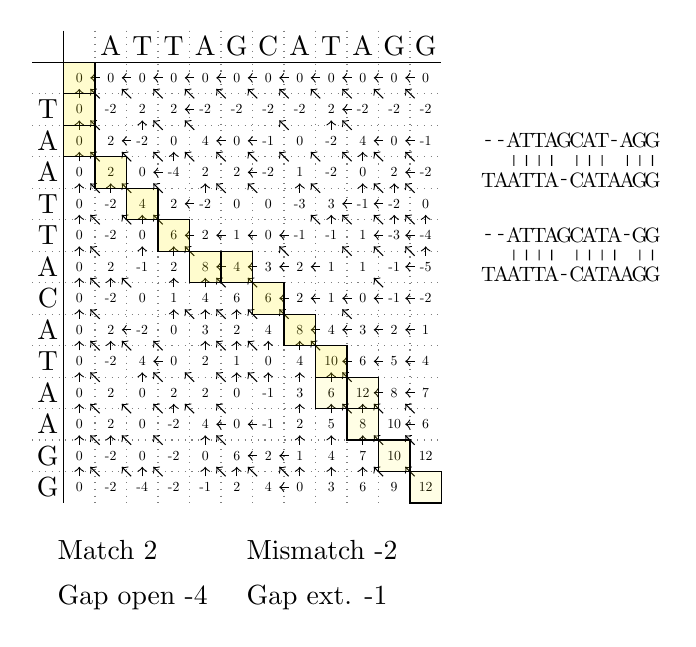
\begin{tikzpicture}[scale=0.4]
      \node [right] at (1,-1) {Match 2};
\node [right] at (7,-1) {Mismatch -2};
\node [right] at (1,-2.5) {Gap open -4};
\node [right] at (7,-2.5) {Gap ext. -1};
\visible<2->{
\draw [-] (0.5,14.5) -- (13.5,14.5);
\draw [-] (1.5,15.5) -- (1.5,0.5);
\draw [-, dotted, opacity=0.5] (0.5,13.5) -- (13.5,13.5);
\draw [-, dotted, opacity=0.5] (2.5,15.5) -- (2.5,0.5);
	\node at (3,15) {A};
	\draw [-, dotted, opacity=0.5] (3.5,15.5) -- (3.5,0.5);
	\node at (4,15) {T};
	\draw [-, dotted, opacity=0.5] (4.5,15.5) -- (4.5,0.5);
	\node at (5,15) {T};
	\draw [-, dotted, opacity=0.5] (5.5,15.5) -- (5.5,0.5);
	\node at (6,15) {A};
	\draw [-, dotted, opacity=0.5] (6.5,15.5) -- (6.5,0.5);
	\node at (7,15) {G};
	\draw [-, dotted, opacity=0.5] (7.5,15.5) -- (7.5,0.5);
	\node at (8,15) {C};
	\draw [-, dotted, opacity=0.5] (8.5,15.5) -- (8.5,0.5);
	\node at (9,15) {A};
	\draw [-, dotted, opacity=0.5] (9.5,15.5) -- (9.5,0.5);
	\node at (10,15) {T};
	\draw [-, dotted, opacity=0.5] (10.5,15.5) -- (10.5,0.5);
	\node at (11,15) {A};
	\draw [-, dotted, opacity=0.5] (11.5,15.5) -- (11.5,0.5);
	\node at (12,15) {G};
	\draw [-, dotted, opacity=0.5] (12.5,15.5) -- (12.5,0.5);
	\node at (13,15) {G};
	\node at (1,13) {T};
	\draw [-, dotted, opacity=0.5] (0.5,12.5) -- (13.5,12.5);
	\node at (1,12) {A};
	\draw [-, dotted, opacity=0.5] (0.5,11.5) -- (13.5,11.5);
	\node at (1,11) {A};
	\draw [-, dotted, opacity=0.5] (0.5,10.5) -- (13.5,10.5);
	\node at (1,10) {T};
	\draw [-, dotted, opacity=0.5] (0.5,9.5) -- (13.5,9.5);
	\node at (1,9) {T};
	\draw [-, dotted, opacity=0.5] (0.5,8.5) -- (13.5,8.5);
	\node at (1,8) {A};
	\draw [-, dotted, opacity=0.5] (0.5,7.5) -- (13.5,7.5);
	\node at (1,7) {C};
	\draw [-, dotted, opacity=0.5] (0.5,6.5) -- (13.5,6.5);
	\node at (1,6) {A};
	\draw [-, dotted, opacity=0.5] (0.5,5.5) -- (13.5,5.5);
	\node at (1,5) {T};
	\draw [-, dotted, opacity=0.5] (0.5,4.5) -- (13.5,4.5);
	\node at (1,4) {A};
	\draw [-, dotted, opacity=0.5] (0.5,3.5) -- (13.5,3.5);
	\node at (1,3) {A};
	\draw [-, dotted, opacity=0.5] (0.5,2.5) -- (13.5,2.5);
	\node at (1,2) {G};
	\draw [-, dotted, opacity=0.5] (0.5,1.5) -- (13.5,1.5);
	\node at (1,1) {G};
}
\visible<3->{
	\node[scale=0.5] at (2,14) {0};
	\node[scale=0.5] at (3,14) {0};
	\draw [->] (2.65, 13+1) -- (2.35, 13+1);
	\node[scale=0.5] at(4,14) {0};
	\draw [->] (3.65,13+1) -- (3.35,13+1);
	\node[scale=0.5] at(5,14) {0};
	\draw [->] (4.65,13+1) -- (4.35,13+1);
	\node[scale=0.5] at(6,14) {0};
	\draw [->] (5.65,13+1) -- (5.35,13+1);
	\node[scale=0.5] at(7,14) {0};
	\draw [->] (6.65,13+1) -- (6.35,13+1);
	\node[scale=0.5] at(8,14) {0};
	\draw [->] (7.65,13+1) -- (7.35,13+1);
	\node[scale=0.5] at(9,14) {0};
	\draw [->] (8.65,13+1) -- (8.35,13+1);
	\node[scale=0.5] at(10,14) {0};
	\draw [->] (9.65,13+1) -- (9.35,13+1);
	\node[scale=0.5] at(11,14) {0};
	\draw [->] (10.65,13+1) -- (10.35,13+1);
	\node[scale=0.5] at(12,14) {0};
	\draw [->] (11.65,13+1) -- (11.35,13+1);
	\node[scale=0.5] at(13,14) {0};
	\draw [->] (12.65,13+1) -- (12.35,13+1);
	\node[scale=0.5] at (2,13) {0};
	\draw [->] (2,13 + 0.35) -- (2, 13 + 0.65);
	\node[scale=0.5] at(2,12) {0};
	\draw [->] (2,13-1 + 0.35) -- (2, 13-1 + 0.65);
	\node[scale=0.5] at(2,11) {0};
	\draw [->] (2,13-2 + 0.35) -- (2, 13-2 + 0.65);
	\node[scale=0.5] at(2,10) {0};
	\draw [->] (2,13-3 + 0.35) -- (2, 13-3 + 0.65);
	\node[scale=0.5] at(2,9) {0};
	\draw [->] (2,13-4 + 0.35) -- (2, 13-4 + 0.65);
	\node[scale=0.5] at(2,8) {0};
	\draw [->] (2,13-5 + 0.35) -- (2, 13-5 + 0.65);
	\node[scale=0.5] at(2,7) {0};
	\draw [->] (2,13-6 + 0.35) -- (2, 13-6 + 0.65);
	\node[scale=0.5] at(2,6) {0};
	\draw [->] (2,13-7 + 0.35) -- (2, 13-7 + 0.65);
	\node[scale=0.5] at(2,5) {0};
	\draw [->] (2,13-8 + 0.35) -- (2, 13-8 + 0.65);
	\node[scale=0.5] at(2,4) {0};
	\draw [->] (2,13-9 + 0.35) -- (2, 13-9 + 0.65);
	\node[scale=0.5] at(2,3) {0};
	\draw [->] (2,13-10 + 0.35) -- (2, 13-10 + 0.65);
	\node[scale=0.5] at(2,2) {0};
	\draw [->] (2,13-11 + 0.35) -- (2, 13-11 + 0.65);
	\node[scale=0.5] at(2,1) {0};
	\draw [->] (2,13-12 + 0.35) -- (2, 13-12 + 0.65);
}
\visible<4->{
	\node [scale=0.5] at (3,13) {-2};
	\draw [->] (2.65,13.35) -- (2.35,13.65);
	\node [scale=0.5] at (4,13) {2};
	\draw [->] (3.65,13.35) -- (3.35,13.65);
	\node [scale=0.5] at (5,13) {2};
	\draw [->] (4.65,13.35) -- (4.35,13.65);
	\node [scale=0.5] at (6,13) {-2};
	\draw [->] (5.65,13.35) -- (5.35,13.65);
	\draw [->] (5.65,13) -- (5.35,13);
	\node [scale=0.5] at (7,13) {-2};
	\draw [->] (6.65,13.35) -- (6.35,13.65);
	\node [scale=0.5] at (8,13) {-2};
	\draw [->] (7.65,13.35) -- (7.35,13.65);
	\node [scale=0.5] at (9,13) {-2};
	\draw [->] (8.65,13.35) -- (8.35,13.65);
	\node [scale=0.5] at (10,13) {2};
	\draw [->] (9.65,13.35) -- (9.35,13.65);
	\node [scale=0.5] at (11,13) {-2};
	\draw [->] (10.65,13.35) -- (10.35,13.65);
	\draw [->] (10.65,13) -- (10.35,13);
	\node [scale=0.5] at (12,13) {-2};
	\draw [->] (11.65,13.35) -- (11.35,13.65);
	\node [scale=0.5] at (13,13) {-2};
	\draw [->] (12.65,13.35) -- (12.35,13.65);
}
\visible<5->{
	\node [scale=0.5] at (3,12) {2};
	\draw [->] (2.65,12.35) -- (2.35,12.65);
	\node [scale=0.5] at (4,12) {-2};
	\draw [->] (3.65,12) -- (3.35,12);
	\draw [->] (4,12.35) -- (4,12.65);
	\node [scale=0.5] at (5,12) {0};
	\draw [->] (4.65,12.35) -- (4.35,12.65);
	\node [scale=0.5] at (6,12) {4};
	\draw [->] (5.65,12.35) -- (5.35,12.65);
	\node [scale=0.5] at (7,12) {0};
	\draw [->] (6.65,12) -- (6.35,12);
	\node [scale=0.5] at (8,12) {-1};
	\draw [->] (7.65,12) -- (7.35,12);
	\node [scale=0.5] at (9,12) {0};
	\draw [->] (8.65,12.35) -- (8.35,12.65);
	\node [scale=0.5] at (10,12) {-2};
	\draw [->] (10,12.35) -- (10,12.65);
	\node [scale=0.5] at (11,12) {4};
	\draw [->] (10.65,12.35) -- (10.35,12.65);
	\node [scale=0.5] at (12,12) {0};
	\draw [->] (11.65,12) -- (11.35,12);
	\node [scale=0.5] at (13,12) {-1};
	\draw [->] (12.65,12) -- (12.35,12);
}
\visible<6->{
	\node [scale=0.5] at (3,11) {2};
	\draw [->] (2.65,11.35) -- (2.35,11.65);
	\node [scale=0.5] at (4,11) {0};
	\draw [->] (3.65,11.35) -- (3.35,11.65);
	\node [scale=0.5] at (5,11) {-4};
	\draw [->] (4.65,11.35) -- (4.35,11.65);
	\draw [->] (4.65,11) -- (4.35,11);
	\draw [->] (5,11.35) -- (5,11.65);
	\node [scale=0.5] at (6,11) {2};
	\draw [->] (5.65,11.35) -- (5.35,11.65);
	\node [scale=0.5] at (7,11) {2};
	\draw [->] (6.65,11.35) -- (6.35,11.65);
	\node [scale=0.5] at (8,11) {-2};
	\draw [->] (7.65,11.35) -- (7.35,11.65);
	\draw [->] (7.65,11) -- (7.35,11);
	\node [scale=0.5] at (9,11) {1};
	\draw [->] (8.65,11.35) -- (8.35,11.65);
	\node [scale=0.5] at (10,11) {-2};
	\draw [->] (9.65,11.35) -- (9.35,11.65);
	\node [scale=0.5] at (11,11) {0};
	\draw [->] (10.65,11.35) -- (10.35,11.65);
	\draw [->] (11,11.35) -- (11,11.65);
	\node [scale=0.5] at (12,11) {2};
	\draw [->] (11.65,11.35) -- (11.35,11.65);
	\node [scale=0.5] at (13,11) {-2};
	\draw [->] (12.65,11.35) -- (12.35,11.65);
	\draw [->] (12.65,11) -- (12.35,11);
}
\visible<7->{
	\node [scale=0.5] at (3,10) {-2};
	\draw [->] (2.65,10.35) -- (2.35,10.65);
	\draw [->] (3,10.35) -- (3,10.65);
	\node [scale=0.5] at (4,10) {4};
	\draw [->] (3.65,10.35) -- (3.35,10.65);
	\node [scale=0.5] at (5,10) {2};
	\draw [->] (4.65,10.35) -- (4.35,10.65);
	\node [scale=0.5] at (6,10) {-2};
	\draw [->] (5.65,10) -- (5.35,10);
	\draw [->] (6,10.35) -- (6,10.65);
	\node [scale=0.5] at (7,10) {0};
	\draw [->] (6.65,10.35) -- (6.35,10.65);
	\node [scale=0.5] at (8,10) {0};
	\draw [->] (7.65,10.35) -- (7.35,10.65);
	\node [scale=0.5] at (9,10) {-3};
	\draw [->] (9,10.35) -- (9,10.65);
	\node [scale=0.5] at (10,10) {3};
	\draw [->] (9.65,10.35) -- (9.35,10.65);
	\node [scale=0.5] at (11,10) {-1};
	\draw [->] (10.65,10) -- (10.35,10);
	\draw [->] (11,10.35) -- (11,10.65);
	\node [scale=0.5] at (12,10) {-2};
	\draw [->] (11.65,10.35) -- (11.35,10.65);
	\draw [->] (11.65,10) -- (11.35,10);
	\draw [->] (12,10.35) -- (12,10.65);
	\node [scale=0.5] at (13,10) {0};
	\draw [->] (12.65,10.35) -- (12.35,10.65);
}
\visible<8->{
	\node [scale=0.5] at (3,9) {-2};
	\draw [->] (2.65,9.35) -- (2.35,9.65);
	\node [scale=0.5] at (4,9) {0};
	\draw [->] (3.65,9.35) -- (3.35,9.65);
	\draw [->] (4,9.35) -- (4,9.65);
	\node [scale=0.5] at (5,9) {6};
	\draw [->] (4.65,9.35) -- (4.35,9.65);
	\node [scale=0.5] at (6,9) {2};
	\draw [->] (5.65,9) -- (5.35,9);
	\node [scale=0.5] at (7,9) {1};
	\draw [->] (6.65,9) -- (6.35,9);
	\node [scale=0.5] at (8,9) {0};
	\draw [->] (7.65,9) -- (7.35,9);
	\node [scale=0.5] at (9,9) {-1};
	\draw [->] (8.65,9) -- (8.35,9);
	\node [scale=0.5] at (10,9) {-1};
	\draw [->] (9.65,9.35) -- (9.35,9.65);
	\draw [->] (10,9.35) -- (10,9.65);
	\node [scale=0.5] at (11,9) {1};
	\draw [->] (10.65,9.35) -- (10.35,9.65);
	\node [scale=0.5] at (12,9) {-3};
	\draw [->] (11.65,9.35) -- (11.35,9.65);
	\draw [->] (11.65,9) -- (11.35,9);
	\draw [->] (12,9.35) -- (12,9.65);
	\node [scale=0.5] at (13,9) {-4};
	\draw [->] (12.65,9.35) -- (12.35,9.65);
	\draw [->] (12.65,9) -- (12.35,9);
	\draw [->] (13,9.35) -- (13,9.65);
}
\visible<9->{
	\node [scale=0.5] at (3,8) {2};
	\draw [->] (2.65,8.35) -- (2.35,8.65);
	\node [scale=0.5] at (4,8) {-1};
	\draw [->] (4,8.35) -- (4,8.65);
	\node [scale=0.5] at (5,8) {2};
	\draw [->] (5,8.35) -- (5,8.65);
	\node [scale=0.5] at (6,8) {8};
	\draw [->] (5.65,8.35) -- (5.35,8.65);
	\node [scale=0.5] at (7,8) {4};
	\draw [->] (6.65,8) -- (6.35,8);
	\node [scale=0.5] at (8,8) {3};
	\draw [->] (7.65,8) -- (7.35,8);
	\node [scale=0.5] at (9,8) {2};
	\draw [->] (8.65,8.35) -- (8.35,8.65);
	\draw [->] (8.65,8) -- (8.35,8);
	\node [scale=0.5] at (10,8) {1};
	\draw [->] (9.65,8) -- (9.35,8);
	\node [scale=0.5] at (11,8) {1};
	\draw [->] (10.65,8.35) -- (10.35,8.65);
	\node [scale=0.5] at (12,8) {-1};
	\draw [->] (11.65,8.35) -- (11.35,8.65);
	\node [scale=0.5] at (13,8) {-5};
	\draw [->] (12.65,8.35) -- (12.35,8.65);
	\draw [->] (12.65,8) -- (12.35,8);
	\draw [->] (13,8.35) -- (13,8.65);
}
\visible<10->{
	\node [scale=0.5] at (3,7) {-2};
	\draw [->] (2.65,7.35) -- (2.35,7.65);
	\draw [->] (3,7.35) -- (3,7.65);
	\node [scale=0.5] at (4,7) {0};
	\draw [->] (3.65,7.35) -- (3.35,7.65);
	\node [scale=0.5] at (5,7) {1};
	\draw [->] (5,7.35) -- (5,7.65);
	\node [scale=0.5] at (6,7) {4};
	\draw [->] (6,7.35) -- (6,7.65);
	\node [scale=0.5] at (7,7) {6};
	\draw [->] (6.65,7.35) -- (6.35,7.65);
	\node [scale=0.5] at (8,7) {6};
	\draw [->] (7.65,7.35) -- (7.35,7.65);
	\node [scale=0.5] at (9,7) {2};
	\draw [->] (8.65,7) -- (8.35,7);
	\node [scale=0.5] at (10,7) {1};
	\draw [->] (9.65,7) -- (9.35,7);
	\node [scale=0.5] at (11,7) {0};
	\draw [->] (10.65,7) -- (10.35,7);
	\node [scale=0.5] at (12,7) {-1};
	\draw [->] (11.65,7.35) -- (11.35,7.65);
	\draw [->] (11.65,7) -- (11.35,7);
	\node [scale=0.5] at (13,7) {-2};
	\draw [->] (12.65,7) -- (12.35,7);
}
\visible<11->{
	\node [scale=0.5] at (3,6) {2};
	\draw [->] (2.65,6.35) -- (2.35,6.65);
	\node [scale=0.5] at (4,6) {-2};
	\draw [->] (3.65,6) -- (3.35,6);
	\node [scale=0.5] at (5,6) {0};
	\draw [->] (5,6.35) -- (5,6.65);
	\node [scale=0.5] at (6,6) {3};
	\draw [->] (5.65,6.35) -- (5.35,6.65);
	\draw [->] (6,6.35) -- (6,6.65);
	\node [scale=0.5] at (7,6) {2};
	\draw [->] (6.65,6.35) -- (6.35,6.65);
	\draw [->] (7,6.35) -- (7,6.65);
	\node [scale=0.5] at (8,6) {4};
	\draw [->] (7.65,6.35) -- (7.35,6.65);
	\node [scale=0.5] at (9,6) {8};
	\draw [->] (8.65,6.35) -- (8.35,6.65);
	\node [scale=0.5] at (10,6) {4};
	\draw [->] (9.65,6) -- (9.35,6);
	\node [scale=0.5] at (11,6) {3};
	\draw [->] (10.65,6.35) -- (10.35,6.65);
	\draw [->] (10.65,6) -- (10.35,6);
	\node [scale=0.5] at (12,6) {2};
	\draw [->] (11.65,6) -- (11.35,6);
	\node [scale=0.5] at (13,6) {1};
	\draw [->] (12.65,6) -- (12.35,6);
}
\visible<12->{
	\node [scale=0.5] at (3,5) {-2};
	\draw [->] (2.65,5.35) -- (2.35,5.65);
	\draw [->] (3,5.35) -- (3,5.65);
	\node [scale=0.5] at (4,5) {4};
	\draw [->] (3.65,5.35) -- (3.35,5.65);
	\node [scale=0.5] at (5,5) {0};
	\draw [->] (4.65,5.35) -- (4.35,5.65);
	\draw [->] (4.65,5) -- (4.35,5);
	\node [scale=0.5] at (6,5) {2};
	\draw [->] (6,5.35) -- (6,5.65);
	\node [scale=0.5] at (7,5) {1};
	\draw [->] (6.65,5.35) -- (6.35,5.65);
	\draw [->] (7,5.35) -- (7,5.65);
	\node [scale=0.5] at (8,5) {0};
	\draw [->] (7.65,5.35) -- (7.35,5.65);
	\draw [->] (8,5.35) -- (8,5.65);
	\node [scale=0.5] at (9,5) {4};
	\draw [->] (9,5.35) -- (9,5.65);
	\node [scale=0.5] at (10,5) {10};
	\draw [->] (9.65,5.35) -- (9.35,5.65);
	\node [scale=0.5] at (11,5) {6};
	\draw [->] (10.65,5) -- (10.35,5);
	\node [scale=0.5] at (12,5) {5};
	\draw [->] (11.65,5) -- (11.35,5);
	\node [scale=0.5] at (13,5) {4};
	\draw [->] (12.65,5) -- (12.35,5);
}
\visible<13->{
	\node [scale=0.5] at (3,4) {2};
	\draw [->] (2.65,4.35) -- (2.35,4.65);
	\node [scale=0.5] at (4,4) {0};
	\draw [->] (4,4.35) -- (4,4.65);
	\node [scale=0.5] at (5,4) {2};
	\draw [->] (4.65,4.35) -- (4.35,4.65);
	\node [scale=0.5] at (6,4) {2};
	\draw [->] (5.65,4.35) -- (5.35,4.65);
	\node [scale=0.5] at (7,4) {0};
	\draw [->] (6.65,4.35) -- (6.35,4.65);
	\draw [->] (7,4.35) -- (7,4.65);
	\node [scale=0.5] at (8,4) {-1};
	\draw [->] (7.65,4.35) -- (7.35,4.65);
	\draw [->] (8,4.35) -- (8,4.65);
	\node [scale=0.5] at (9,4) {3};
	\draw [->] (9,4.35) -- (9,4.65);
	\node [scale=0.5] at (10,4) {6};
	\draw [->] (10,4.35) -- (10,4.65);
	\node [scale=0.5] at (11,4) {12};
	\draw [->] (10.65,4.35) -- (10.35,4.65);
	\node [scale=0.5] at (12,4) {8};
	\draw [->] (11.65,4) -- (11.35,4);
	\node [scale=0.5] at (13,4) {7};
	\draw [->] (12.65,4) -- (12.35,4);
}
\visible<14->{
	\node [scale=0.5] at (3,3) {2};
	\draw [->] (2.65,3.35) -- (2.35,3.65);
	\node [scale=0.5] at (4,3) {0};
	\draw [->] (3.65,3.35) -- (3.35,3.65);
	\node [scale=0.5] at (5,3) {-2};
	\draw [->] (4.65,3.35) -- (4.35,3.65);
	\draw [->] (5,3.35) -- (5,3.65);
	\node [scale=0.5] at (6,3) {4};
	\draw [->] (5.65,3.35) -- (5.35,3.65);
	\node [scale=0.5] at (7,3) {0};
	\draw [->] (6.65,3.35) -- (6.35,3.65);
	\draw [->] (6.65,3) -- (6.35,3);
	\node [scale=0.5] at (8,3) {-1};
	\draw [->] (7.65,3) -- (7.35,3);
	\node [scale=0.5] at (9,3) {2};
	\draw [->] (9,3.35) -- (9,3.65);
	\node [scale=0.5] at (10,3) {5};
	\draw [->] (10,3.35) -- (10,3.65);
	\node [scale=0.5] at (11,3) {8};
	\draw [->] (10.65,3.35) -- (10.35,3.65);
	\draw [->] (11,3.35) -- (11,3.65);
	\node [scale=0.5] at (12,3) {10};
	\draw [->] (11.65,3.35) -- (11.35,3.65);
	\node [scale=0.5] at (13,3) {6};
	\draw [->] (12.65,3.35) -- (12.35,3.65);
	\draw [->] (12.65,3) -- (12.35,3);
}
\visible<15->{
	\node [scale=0.5] at (3,2) {-2};
	\draw [->] (2.65,2.35) -- (2.35,2.65);
	\draw [->] (3,2.35) -- (3,2.65);
	\node [scale=0.5] at (4,2) {0};
	\draw [->] (3.65,2.35) -- (3.35,2.65);
	\node [scale=0.5] at (5,2) {-2};
	\draw [->] (4.65,2.35) -- (4.35,2.65);
	\node [scale=0.5] at (6,2) {0};
	\draw [->] (6,2.35) -- (6,2.65);
	\node [scale=0.5] at (7,2) {6};
	\draw [->] (6.65,2.35) -- (6.35,2.65);
	\node [scale=0.5] at (8,2) {2};
	\draw [->] (7.65,2) -- (7.35,2);
	\node [scale=0.5] at (9,2) {1};
	\draw [->] (8.65,2) -- (8.35,2);
	\draw [->] (9,2.35) -- (9,2.65);
	\node [scale=0.5] at (10,2) {4};
	\draw [->] (10,2.35) -- (10,2.65);
	\node [scale=0.5] at (11,2) {7};
	\draw [->] (11,2.35) -- (11,2.65);
	\node [scale=0.5] at (12,2) {10};
	\draw [->] (11.65,2.35) -- (11.35,2.65);
	\node [scale=0.5] at (13,2) {12};
	\draw [->] (12.65,2.35) -- (12.35,2.65);
}
\visible<16->{
	\node [scale=0.5] at (3,1) {-2};
	\draw [->] (2.65,1.35) -- (2.35,1.65);
	\node [scale=0.5] at (4,1) {-4};
	\draw [->] (3.65,1.35) -- (3.35,1.65);
	\draw [->] (4,1.35) -- (4,1.65);
	\node [scale=0.5] at (5,1) {-2};
	\draw [->] (4.65,1.35) -- (4.35,1.65);
	\node [scale=0.5] at (6,1) {-1};
	\draw [->] (6,1.35) -- (6,1.65);
	\node [scale=0.5] at (7,1) {2};
	\draw [->] (6.65,1.35) -- (6.35,1.65);
	\draw [->] (7,1.35) -- (7,1.65);
	\node [scale=0.5] at (8,1) {4};
	\draw [->] (7.65,1.35) -- (7.35,1.65);
	\node [scale=0.5] at (9,1) {0};
	\draw [->] (8.65,1.35) -- (8.35,1.65);
	\draw [->] (8.65,1) -- (8.35,1);
	\draw [->] (9,1.35) -- (9,1.65);
	\node [scale=0.5] at (10,1) {3};
	\draw [->] (10,1.35) -- (10,1.65);
	\node [scale=0.5] at (11,1) {6};
	\draw [->] (11,1.35) -- (11,1.65);
	\node [scale=0.5] at (12,1) {9};
	\draw [->] (11.65,1.35) -- (11.35,1.65);
	\node [scale=0.5] at (13,1) {12};
	\draw [->] (12.65,1.35) -- (12.35,1.65);
}
\visible<17->{
\draw [fill=yellow, fill opacity=0.1] (12.5,0.5) rectangle (13.5,1.5);
}
\visible<18->{
\draw [fill=yellow, fill opacity=0.1] (11.5,1.5) rectangle (12.5,2.5);
}
\visible<19->{
\draw [fill=yellow, fill opacity=0.1] (10.5,2.5) rectangle (11.5,3.5);
}
\visible<20->{
\draw [fill=yellow, fill opacity=0.1] (9.5,3.5) rectangle (10.5,4.5);
}
\visible<21->{
\draw [fill=yellow, fill opacity=0.1] (9.5,4.5) rectangle (10.5,5.5);
}
\visible<22->{
\draw [fill=yellow, fill opacity=0.1] (8.5,5.5) rectangle (9.5,6.5);
}
\visible<23->{
\draw [fill=yellow, fill opacity=0.1] (7.5,6.5) rectangle (8.5,7.5);
}
\visible<24->{
\draw [fill=yellow, fill opacity=0.1] (6.5,7.5) rectangle (7.5,8.5);
}
\visible<25->{
\draw [fill=yellow, fill opacity=0.1] (5.5,7.5) rectangle (6.5,8.5);
}
\visible<26->{
\draw [fill=yellow, fill opacity=0.1] (4.5,8.5) rectangle (5.5,9.5);
}
\visible<27->{
\draw [fill=yellow, fill opacity=0.1] (3.5,9.5) rectangle (4.5,10.5);
}
\visible<28->{
\draw [fill=yellow, fill opacity=0.1] (2.5,10.5) rectangle (3.5,11.5);
}
\visible<29->{
\draw [fill=yellow, fill opacity=0.1] (1.5,11.5) rectangle (2.5,12.5);
}
\visible<30->{
\draw [fill=yellow, fill opacity=0.1] (1.5,12.5) rectangle (2.5,13.5);
}
\visible<31->{
\draw [fill=yellow, fill opacity=0.1] (1.5,13.5) rectangle (2.5,14.5);
}
\visible<32->{
\draw [fill=yellow, fill opacity=0.1] (10.5,3.5) rectangle (11.5,4.5);
}
\visible<33->{
\draw [fill=yellow, fill opacity=0.1] (9.5,4.5) rectangle (10.5,5.5);
}
\visible<34->{
\draw [fill=yellow, fill opacity=0.1] (8.5,5.5) rectangle (9.5,6.5);
}
\visible<35->{
\draw [fill=yellow, fill opacity=0.1] (7.5,6.5) rectangle (8.5,7.5);
}
\visible<36->{
\draw [fill=yellow, fill opacity=0.1] (6.5,7.5) rectangle (7.5,8.5);
}
\visible<37->{
\draw [fill=yellow, fill opacity=0.1] (5.5,7.5) rectangle (6.5,8.5);
}
\visible<38->{
\draw [fill=yellow, fill opacity=0.1] (4.5,8.5) rectangle (5.5,9.5);
}
\visible<39->{
\draw [fill=yellow, fill opacity=0.1] (3.5,9.5) rectangle (4.5,10.5);
}
\visible<40->{
\draw [fill=yellow, fill opacity=0.1] (2.5,10.5) rectangle (3.5,11.5);
}
\visible<41->{
\draw [fill=yellow, fill opacity=0.1] (1.5,11.5) rectangle (2.5,12.5);
}
\visible<42->{
\draw [fill=yellow, fill opacity=0.1] (1.5,12.5) rectangle (2.5,13.5);
}
\visible<43->{
\draw [fill=yellow, fill opacity=0.1] (1.5,13.5) rectangle (2.5,14.5);
}
\visible<44->{
\node [scale=0.75] (s1) at (15 + 0/2.5, 12) {-};
\node [scale=0.75] (s2) at (15 + 0/2.5, 12-1.25) {T};
\node [scale=0.75] (s1) at (15 + 1/2.5, 12) {-};
\node [scale=0.75] (s2) at (15 + 1/2.5, 12-1.25) {A};
\node [scale=0.75] (s1) at (15 + 2/2.5, 12) {A};
\node [scale=0.75] (s2) at (15 + 2/2.5, 12-1.25) {A};
\draw [-] (s1) -- (s2);
\node [scale=0.75] (s1) at (15 + 3/2.5, 12) {T};
\node [scale=0.75] (s2) at (15 + 3/2.5, 12-1.25) {T};
\draw [-] (s1) -- (s2);
\node [scale=0.75] (s1) at (15 + 4/2.5, 12) {T};
\node [scale=0.75] (s2) at (15 + 4/2.5, 12-1.25) {T};
\draw [-] (s1) -- (s2);
\node [scale=0.75] (s1) at (15 + 5/2.5, 12) {A};
\node [scale=0.75] (s2) at (15 + 5/2.5, 12-1.25) {A};
\draw [-] (s1) -- (s2);
\node [scale=0.75] (s1) at (15 + 6/2.5, 12) {G};
\node [scale=0.75] (s2) at (15 + 6/2.5, 12-1.25) {-};
\node [scale=0.75] (s1) at (15 + 7/2.5, 12) {C};
\node [scale=0.75] (s2) at (15 + 7/2.5, 12-1.25) {C};
\draw [-] (s1) -- (s2);
\node [scale=0.75] (s1) at (15 + 8/2.5, 12) {A};
\node [scale=0.75] (s2) at (15 + 8/2.5, 12-1.25) {A};
\draw [-] (s1) -- (s2);
\node [scale=0.75] (s1) at (15 + 9/2.5, 12) {T};
\node [scale=0.75] (s2) at (15 + 9/2.5, 12-1.25) {T};
\draw [-] (s1) -- (s2);
\node [scale=0.75] (s1) at (15 + 10/2.5, 12) {-};
\node [scale=0.75] (s2) at (15 + 10/2.5, 12-1.25) {A};
\node [scale=0.75] (s1) at (15 + 11/2.5, 12) {A};
\node [scale=0.75] (s2) at (15 + 11/2.5, 12-1.25) {A};
\draw [-] (s1) -- (s2);
\node [scale=0.75] (s1) at (15 + 12/2.5, 12) {G};
\node [scale=0.75] (s2) at (15 + 12/2.5, 12-1.25) {G};
\draw [-] (s1) -- (s2);
\node [scale=0.75] (s1) at (15 + 13/2.5, 12) {G};
\node [scale=0.75] (s2) at (15 + 13/2.5, 12-1.25) {G};
\draw [-] (s1) -- (s2);
\node [scale=0.75] (s1) at (15 + 0/2.5, 9) {-};
\node [scale=0.75] (s2) at (15 + 0/2.5, 9-1.25) {T};
\node [scale=0.75] (s1) at (15 + 1/2.5, 9) {-};
\node [scale=0.75] (s2) at (15 + 1/2.5, 9-1.25) {A};
\node [scale=0.75] (s1) at (15 + 2/2.5, 9) {A};
\node [scale=0.75] (s2) at (15 + 2/2.5, 9-1.25) {A};
\draw [-] (s1) -- (s2);
\node [scale=0.75] (s1) at (15 + 3/2.5, 9) {T};
\node [scale=0.75] (s2) at (15 + 3/2.5, 9-1.25) {T};
\draw [-] (s1) -- (s2);
\node [scale=0.75] (s1) at (15 + 4/2.5, 9) {T};
\node [scale=0.75] (s2) at (15 + 4/2.5, 9-1.25) {T};
\draw [-] (s1) -- (s2);
\node [scale=0.75] (s1) at (15 + 5/2.5, 9) {A};
\node [scale=0.75] (s2) at (15 + 5/2.5, 9-1.25) {A};
\draw [-] (s1) -- (s2);
\node [scale=0.75] (s1) at (15 + 6/2.5, 9) {G};
\node [scale=0.75] (s2) at (15 + 6/2.5, 9-1.25) {-};
\node [scale=0.75] (s1) at (15 + 7/2.5, 9) {C};
\node [scale=0.75] (s2) at (15 + 7/2.5, 9-1.25) {C};
\draw [-] (s1) -- (s2);
\node [scale=0.75] (s1) at (15 + 8/2.5, 9) {A};
\node [scale=0.75] (s2) at (15 + 8/2.5, 9-1.25) {A};
\draw [-] (s1) -- (s2);
\node [scale=0.75] (s1) at (15 + 9/2.5, 9) {T};
\node [scale=0.75] (s2) at (15 + 9/2.5, 9-1.25) {T};
\draw [-] (s1) -- (s2);
\node [scale=0.75] (s1) at (15 + 10/2.5, 9) {A};
\node [scale=0.75] (s2) at (15 + 10/2.5, 9-1.25) {A};
\draw [-] (s1) -- (s2);
\node [scale=0.75] (s1) at (15 + 11/2.5, 9) {-};
\node [scale=0.75] (s2) at (15 + 11/2.5, 9-1.25) {A};
\node [scale=0.75] (s1) at (15 + 12/2.5, 9) {G};
\node [scale=0.75] (s2) at (15 + 12/2.5, 9-1.25) {G};
\draw [-] (s1) -- (s2);
\node [scale=0.75] (s1) at (15 + 13/2.5, 9) {G};
\node [scale=0.75] (s2) at (15 + 13/2.5, 9-1.25) {G};
\draw [-] (s1) -- (s2);
}

    \end{tikzpicture}
  \end{figure}
\end{frame}


\begin{frame}[fragile]{Why local alignment?}
  \begin{itemize}
  \item Evolutionary constraints on sequences are variable.
    \begin{description}
    \item[Proteins] Active sites vs connecting loops.
    \item[DNA] Introns vs. Exonic sequences.
    \end{description}
  \item Rearrangements of (insertions/inversions/deletions) homologous
    sequences.
  \end{itemize}
  
  This means two sequences can contain islands of homology connected
  by non-homologous regions, or regions of homology in a rearranged order. eg:

  A-B-C-D-E $\Rightarrow$ A-C-B-E\\

  {\footnotesize Individual letters indicate a region of homology. An inversion of
    the A-B region and a loss of the D region leads to two sequences which can not
    be meaningfully globally aligned. }

\end{frame}

\begin{frame}{Smith-Waterman: local alignment}
  Smith-Waterman is identical to Needleman-Wunsch except:
  \begin{itemize}
  \item Negative scores are converted to 0 and there are no
    paths from such cells.
  \item The alignment is obtained by starting at the highest
    scoring cell and ends before a 0 valued cell is reached.
  \item Subalignments can start from several points if more than a single
    maximum is obtained.
  \item Non-overlapping sub-alignments can be identified across a sequence.
  \end{itemize}
\end{frame}

\begin{frame}{Smith-Waterman: local alignment}
  \begin{figure}[ht]
    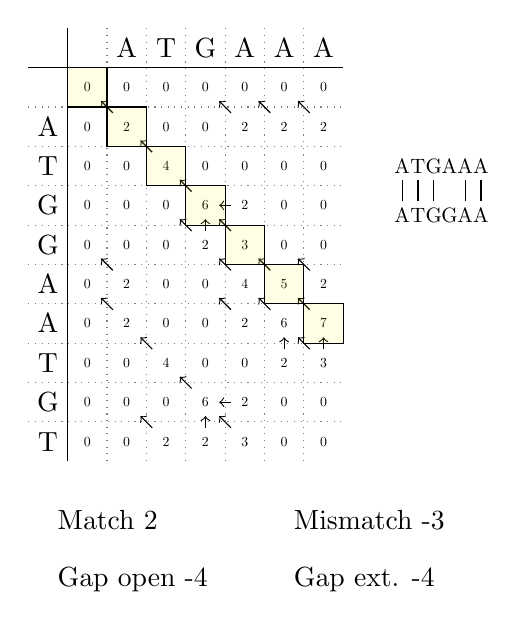
\begin{tikzpicture}[scale=0.5]
      \node [right] at (1,-1) {Match 2};
\node [right] at (7,-1) {Mismatch -3};
\node [right] at (1,-2.5) {Gap open -4};
\node [right] at (7,-2.5) {Gap ext. -4};
\visible<2->{
\draw [-] (0.5,10.5) -- (8.5,10.5);
\draw [-] (1.5,11.5) -- (1.5,0.5);
\draw [-, dotted, opacity=0.5] (0.5,9.5) -- (8.5,9.5);
\draw [-, dotted, opacity=0.5] (2.5,11.5) -- (2.5,0.5);
	\node at (3,11) {A};
	\draw [-, dotted, opacity=0.5] (3.5,11.5) -- (3.5,0.5);
	\node at (4,11) {T};
	\draw [-, dotted, opacity=0.5] (4.5,11.5) -- (4.5,0.5);
	\node at (5,11) {G};
	\draw [-, dotted, opacity=0.5] (5.5,11.5) -- (5.5,0.5);
	\node at (6,11) {A};
	\draw [-, dotted, opacity=0.5] (6.5,11.5) -- (6.5,0.5);
	\node at (7,11) {A};
	\draw [-, dotted, opacity=0.5] (7.5,11.5) -- (7.5,0.5);
	\node at (8,11) {A};
	\node at (1,9) {A};
	\draw [-, dotted, opacity=0.5] (0.5,8.5) -- (8.5,8.5);
	\node at (1,8) {T};
	\draw [-, dotted, opacity=0.5] (0.5,7.5) -- (8.5,7.5);
	\node at (1,7) {G};
	\draw [-, dotted, opacity=0.5] (0.5,6.5) -- (8.5,6.5);
	\node at (1,6) {G};
	\draw [-, dotted, opacity=0.5] (0.5,5.5) -- (8.5,5.5);
	\node at (1,5) {A};
	\draw [-, dotted, opacity=0.5] (0.5,4.5) -- (8.5,4.5);
	\node at (1,4) {A};
	\draw [-, dotted, opacity=0.5] (0.5,3.5) -- (8.5,3.5);
	\node at (1,3) {T};
	\draw [-, dotted, opacity=0.5] (0.5,2.5) -- (8.5,2.5);
	\node at (1,2) {G};
	\draw [-, dotted, opacity=0.5] (0.5,1.5) -- (8.5,1.5);
	\node at (1,1) {T};
}
\visible<3->{
	\node[scale=0.5] at (2,10) {0};
	\node[scale=0.5] at (3,10) {0};
	\node[scale=0.5] at(4,10) {0};
	\node[scale=0.5] at(5,10) {0};
	\node[scale=0.5] at(6,10) {0};
	\node[scale=0.5] at(7,10) {0};
	\node[scale=0.5] at(8,10) {0};
	\node[scale=0.5] at (2,9) {0};
	\node[scale=0.5] at(2,8) {0};
	\node[scale=0.5] at(2,7) {0};
	\node[scale=0.5] at(2,6) {0};
	\node[scale=0.5] at(2,5) {0};
	\node[scale=0.5] at(2,4) {0};
	\node[scale=0.5] at(2,3) {0};
	\node[scale=0.5] at(2,2) {0};
	\node[scale=0.5] at(2,1) {0};
}
\visible<4->{
	\node [scale=0.5] at (3,9) {2};
	\draw [->] (2.65,9.35) -- (2.35,9.65);
	\node [scale=0.5] at (4,9) {0};
	\node [scale=0.5] at (5,9) {0};
	\node [scale=0.5] at (6,9) {2};
	\draw [->] (5.65,9.35) -- (5.35,9.65);
	\node [scale=0.5] at (7,9) {2};
	\draw [->] (6.65,9.35) -- (6.35,9.65);
	\node [scale=0.5] at (8,9) {2};
	\draw [->] (7.65,9.35) -- (7.35,9.65);
}
\visible<5->{
	\node [scale=0.5] at (3,8) {0};
	\node [scale=0.5] at (4,8) {4};
	\draw [->] (3.65,8.35) -- (3.35,8.65);
	\node [scale=0.5] at (5,8) {0};
	\node [scale=0.5] at (6,8) {0};
	\node [scale=0.5] at (7,8) {0};
	\node [scale=0.5] at (8,8) {0};
}
\visible<6->{
	\node [scale=0.5] at (3,7) {0};
	\node [scale=0.5] at (4,7) {0};
	\node [scale=0.5] at (5,7) {6};
	\draw [->] (4.65,7.35) -- (4.35,7.65);
	\node [scale=0.5] at (6,7) {2};
	\draw [->] (5.65,7) -- (5.35,7);
	\node [scale=0.5] at (7,7) {0};
	\node [scale=0.5] at (8,7) {0};
}
\visible<7->{
	\node [scale=0.5] at (3,6) {0};
	\node [scale=0.5] at (4,6) {0};
	\node [scale=0.5] at (5,6) {2};
	\draw [->] (4.65,6.35) -- (4.35,6.65);
	\draw [->] (5,6.35) -- (5,6.65);
	\node [scale=0.5] at (6,6) {3};
	\draw [->] (5.65,6.35) -- (5.35,6.65);
	\node [scale=0.5] at (7,6) {0};
	\node [scale=0.5] at (8,6) {0};
}
\visible<8->{
	\node [scale=0.5] at (3,5) {2};
	\draw [->] (2.65,5.35) -- (2.35,5.65);
	\node [scale=0.5] at (4,5) {0};
	\node [scale=0.5] at (5,5) {0};
	\node [scale=0.5] at (6,5) {4};
	\draw [->] (5.65,5.35) -- (5.35,5.65);
	\node [scale=0.5] at (7,5) {5};
	\draw [->] (6.65,5.35) -- (6.35,5.65);
	\node [scale=0.5] at (8,5) {2};
	\draw [->] (7.65,5.35) -- (7.35,5.65);
}
\visible<9->{
	\node [scale=0.5] at (3,4) {2};
	\draw [->] (2.65,4.35) -- (2.35,4.65);
	\node [scale=0.5] at (4,4) {0};
	\node [scale=0.5] at (5,4) {0};
	\node [scale=0.5] at (6,4) {2};
	\draw [->] (5.65,4.35) -- (5.35,4.65);
	\node [scale=0.5] at (7,4) {6};
	\draw [->] (6.65,4.35) -- (6.35,4.65);
	\node [scale=0.5] at (8,4) {7};
	\draw [->] (7.65,4.35) -- (7.35,4.65);
}
\visible<10->{
	\node [scale=0.5] at (3,3) {0};
	\node [scale=0.5] at (4,3) {4};
	\draw [->] (3.65,3.35) -- (3.35,3.65);
	\node [scale=0.5] at (5,3) {0};
	\node [scale=0.5] at (6,3) {0};
	\node [scale=0.5] at (7,3) {2};
	\draw [->] (7,3.35) -- (7,3.65);
	\node [scale=0.5] at (8,3) {3};
	\draw [->] (7.65,3.35) -- (7.35,3.65);
	\draw [->] (8,3.35) -- (8,3.65);
}
\visible<11->{
	\node [scale=0.5] at (3,2) {0};
	\node [scale=0.5] at (4,2) {0};
	\node [scale=0.5] at (5,2) {6};
	\draw [->] (4.65,2.35) -- (4.35,2.65);
	\node [scale=0.5] at (6,2) {2};
	\draw [->] (5.65,2) -- (5.35,2);
	\node [scale=0.5] at (7,2) {0};
	\node [scale=0.5] at (8,2) {0};
}
\visible<12->{
	\node [scale=0.5] at (3,1) {0};
	\node [scale=0.5] at (4,1) {2};
	\draw [->] (3.65,1.35) -- (3.35,1.65);
	\node [scale=0.5] at (5,1) {2};
	\draw [->] (5,1.35) -- (5,1.65);
	\node [scale=0.5] at (6,1) {3};
	\draw [->] (5.65,1.35) -- (5.35,1.65);
	\node [scale=0.5] at (7,1) {0};
	\node [scale=0.5] at (8,1) {0};
}
\visible<13->{
\draw [fill=yellow, fill opacity=0.1] (7.5,3.5) rectangle (8.5,4.5);
}
\visible<14->{
\draw [fill=yellow, fill opacity=0.1] (6.5,4.5) rectangle (7.5,5.5);
}
\visible<15->{
\draw [fill=yellow, fill opacity=0.1] (5.5,5.5) rectangle (6.5,6.5);
}
\visible<16->{
\draw [fill=yellow, fill opacity=0.1] (4.5,6.5) rectangle (5.5,7.5);
}
\visible<17->{
\draw [fill=yellow, fill opacity=0.1] (3.5,7.5) rectangle (4.5,8.5);
}
\visible<18->{
\draw [fill=yellow, fill opacity=0.1] (2.5,8.5) rectangle (3.5,9.5);
}
\visible<19->{
\draw [fill=yellow, fill opacity=0.1] (1.5,9.5) rectangle (2.5,10.5);
}
\visible<20->{
\node [scale=0.75] (s1) at (10 + 0/2.5, 8) {A};
\node [scale=0.75] (s2) at (10 + 0/2.5, 8-1.25) {A};
\draw [-] (s1) -- (s2);
\node [scale=0.75] (s1) at (10 + 1/2.5, 8) {T};
\node [scale=0.75] (s2) at (10 + 1/2.5, 8-1.25) {T};
\draw [-] (s1) -- (s2);
\node [scale=0.75] (s1) at (10 + 2/2.5, 8) {G};
\node [scale=0.75] (s2) at (10 + 2/2.5, 8-1.25) {G};
\draw [-] (s1) -- (s2);
\node [scale=0.75] (s1) at (10 + 3/2.5, 8) {A};
\node [scale=0.75] (s2) at (10 + 3/2.5, 8-1.25) {G};
\node [scale=0.75] (s1) at (10 + 4/2.5, 8) {A};
\node [scale=0.75] (s2) at (10 + 4/2.5, 8-1.25) {A};
\draw [-] (s1) -- (s2);
\node [scale=0.75] (s1) at (10 + 5/2.5, 8) {A};
\node [scale=0.75] (s2) at (10 + 5/2.5, 8-1.25) {A};
\draw [-] (s1) -- (s2);
}

    \end{tikzpicture}
  \end{figure}
\end{frame}

\begin{frame}{Smith-Waterman: local alignment (2)}
  \begin{figure}[ht]
    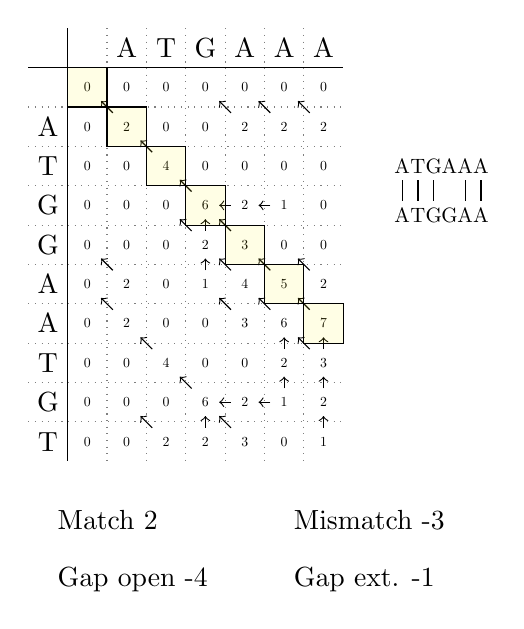
\begin{tikzpicture}[scale=0.5]
      \node [right] at (1,-1) {Match 2};
\node [right] at (7,-1) {Mismatch -3};
\node [right] at (1,-2.5) {Gap open -4};
\node [right] at (7,-2.5) {Gap ext. -1};
\visible<2->{
\draw [-] (0.5,10.5) -- (8.5,10.5);
\draw [-] (1.5,11.5) -- (1.5,0.5);
\draw [-, dotted, opacity=0.5] (0.5,9.5) -- (8.5,9.5);
\draw [-, dotted, opacity=0.5] (2.5,11.5) -- (2.5,0.5);
	\node at (3,11) {A};
	\draw [-, dotted, opacity=0.5] (3.5,11.5) -- (3.5,0.5);
	\node at (4,11) {T};
	\draw [-, dotted, opacity=0.5] (4.5,11.5) -- (4.5,0.5);
	\node at (5,11) {G};
	\draw [-, dotted, opacity=0.5] (5.5,11.5) -- (5.5,0.5);
	\node at (6,11) {A};
	\draw [-, dotted, opacity=0.5] (6.5,11.5) -- (6.5,0.5);
	\node at (7,11) {A};
	\draw [-, dotted, opacity=0.5] (7.5,11.5) -- (7.5,0.5);
	\node at (8,11) {A};
	\node at (1,9) {A};
	\draw [-, dotted, opacity=0.5] (0.5,8.5) -- (8.5,8.5);
	\node at (1,8) {T};
	\draw [-, dotted, opacity=0.5] (0.5,7.5) -- (8.5,7.5);
	\node at (1,7) {G};
	\draw [-, dotted, opacity=0.5] (0.5,6.5) -- (8.5,6.5);
	\node at (1,6) {G};
	\draw [-, dotted, opacity=0.5] (0.5,5.5) -- (8.5,5.5);
	\node at (1,5) {A};
	\draw [-, dotted, opacity=0.5] (0.5,4.5) -- (8.5,4.5);
	\node at (1,4) {A};
	\draw [-, dotted, opacity=0.5] (0.5,3.5) -- (8.5,3.5);
	\node at (1,3) {T};
	\draw [-, dotted, opacity=0.5] (0.5,2.5) -- (8.5,2.5);
	\node at (1,2) {G};
	\draw [-, dotted, opacity=0.5] (0.5,1.5) -- (8.5,1.5);
	\node at (1,1) {T};
}
\visible<3->{
	\node[scale=0.5] at (2,10) {0};
	\node[scale=0.5] at (3,10) {0};
	\node[scale=0.5] at(4,10) {0};
	\node[scale=0.5] at(5,10) {0};
	\node[scale=0.5] at(6,10) {0};
	\node[scale=0.5] at(7,10) {0};
	\node[scale=0.5] at(8,10) {0};
	\node[scale=0.5] at (2,9) {0};
	\node[scale=0.5] at(2,8) {0};
	\node[scale=0.5] at(2,7) {0};
	\node[scale=0.5] at(2,6) {0};
	\node[scale=0.5] at(2,5) {0};
	\node[scale=0.5] at(2,4) {0};
	\node[scale=0.5] at(2,3) {0};
	\node[scale=0.5] at(2,2) {0};
	\node[scale=0.5] at(2,1) {0};
}
\visible<4->{
	\node [scale=0.5] at (3,9) {2};
	\draw [->] (2.65,9.35) -- (2.35,9.65);
	\node [scale=0.5] at (4,9) {0};
	\node [scale=0.5] at (5,9) {0};
	\node [scale=0.5] at (6,9) {2};
	\draw [->] (5.65,9.35) -- (5.35,9.65);
	\node [scale=0.5] at (7,9) {2};
	\draw [->] (6.65,9.35) -- (6.35,9.65);
	\node [scale=0.5] at (8,9) {2};
	\draw [->] (7.65,9.35) -- (7.35,9.65);
}
\visible<5->{
	\node [scale=0.5] at (3,8) {0};
	\node [scale=0.5] at (4,8) {4};
	\draw [->] (3.65,8.35) -- (3.35,8.65);
	\node [scale=0.5] at (5,8) {0};
	\node [scale=0.5] at (6,8) {0};
	\node [scale=0.5] at (7,8) {0};
	\node [scale=0.5] at (8,8) {0};
}
\visible<6->{
	\node [scale=0.5] at (3,7) {0};
	\node [scale=0.5] at (4,7) {0};
	\node [scale=0.5] at (5,7) {6};
	\draw [->] (4.65,7.35) -- (4.35,7.65);
	\node [scale=0.5] at (6,7) {2};
	\draw [->] (5.65,7) -- (5.35,7);
	\node [scale=0.5] at (7,7) {1};
	\draw [->] (6.65,7) -- (6.35,7);
	\node [scale=0.5] at (8,7) {0};
}
\visible<7->{
	\node [scale=0.5] at (3,6) {0};
	\node [scale=0.5] at (4,6) {0};
	\node [scale=0.5] at (5,6) {2};
	\draw [->] (4.65,6.35) -- (4.35,6.65);
	\draw [->] (5,6.35) -- (5,6.65);
	\node [scale=0.5] at (6,6) {3};
	\draw [->] (5.65,6.35) -- (5.35,6.65);
	\node [scale=0.5] at (7,6) {0};
	\node [scale=0.5] at (8,6) {0};
}
\visible<8->{
	\node [scale=0.5] at (3,5) {2};
	\draw [->] (2.65,5.35) -- (2.35,5.65);
	\node [scale=0.5] at (4,5) {0};
	\node [scale=0.5] at (5,5) {1};
	\draw [->] (5,5.35) -- (5,5.65);
	\node [scale=0.5] at (6,5) {4};
	\draw [->] (5.65,5.35) -- (5.35,5.65);
	\node [scale=0.5] at (7,5) {5};
	\draw [->] (6.65,5.35) -- (6.35,5.65);
	\node [scale=0.5] at (8,5) {2};
	\draw [->] (7.65,5.35) -- (7.35,5.65);
}
\visible<9->{
	\node [scale=0.5] at (3,4) {2};
	\draw [->] (2.65,4.35) -- (2.35,4.65);
	\node [scale=0.5] at (4,4) {0};
	\node [scale=0.5] at (5,4) {0};
	\node [scale=0.5] at (6,4) {3};
	\draw [->] (5.65,4.35) -- (5.35,4.65);
	\node [scale=0.5] at (7,4) {6};
	\draw [->] (6.65,4.35) -- (6.35,4.65);
	\node [scale=0.5] at (8,4) {7};
	\draw [->] (7.65,4.35) -- (7.35,4.65);
}
\visible<10->{
	\node [scale=0.5] at (3,3) {0};
	\node [scale=0.5] at (4,3) {4};
	\draw [->] (3.65,3.35) -- (3.35,3.65);
	\node [scale=0.5] at (5,3) {0};
	\node [scale=0.5] at (6,3) {0};
	\node [scale=0.5] at (7,3) {2};
	\draw [->] (7,3.35) -- (7,3.65);
	\node [scale=0.5] at (8,3) {3};
	\draw [->] (7.65,3.35) -- (7.35,3.65);
	\draw [->] (8,3.35) -- (8,3.65);
}
\visible<11->{
	\node [scale=0.5] at (3,2) {0};
	\node [scale=0.5] at (4,2) {0};
	\node [scale=0.5] at (5,2) {6};
	\draw [->] (4.65,2.35) -- (4.35,2.65);
	\node [scale=0.5] at (6,2) {2};
	\draw [->] (5.65,2) -- (5.35,2);
	\node [scale=0.5] at (7,2) {1};
	\draw [->] (6.65,2) -- (6.35,2);
	\draw [->] (7,2.35) -- (7,2.65);
	\node [scale=0.5] at (8,2) {2};
	\draw [->] (8,2.35) -- (8,2.65);
}
\visible<12->{
	\node [scale=0.5] at (3,1) {0};
	\node [scale=0.5] at (4,1) {2};
	\draw [->] (3.65,1.35) -- (3.35,1.65);
	\node [scale=0.5] at (5,1) {2};
	\draw [->] (5,1.35) -- (5,1.65);
	\node [scale=0.5] at (6,1) {3};
	\draw [->] (5.65,1.35) -- (5.35,1.65);
	\node [scale=0.5] at (7,1) {0};
	\node [scale=0.5] at (8,1) {1};
	\draw [->] (8,1.35) -- (8,1.65);
}
\visible<13->{
\draw [fill=yellow, fill opacity=0.1] (7.5,3.5) rectangle (8.5,4.5);
}
\visible<14->{
\draw [fill=yellow, fill opacity=0.1] (6.5,4.5) rectangle (7.5,5.5);
}
\visible<15->{
\draw [fill=yellow, fill opacity=0.1] (5.5,5.5) rectangle (6.5,6.5);
}
\visible<16->{
\draw [fill=yellow, fill opacity=0.1] (4.5,6.5) rectangle (5.5,7.5);
}
\visible<17->{
\draw [fill=yellow, fill opacity=0.1] (3.5,7.5) rectangle (4.5,8.5);
}
\visible<18->{
\draw [fill=yellow, fill opacity=0.1] (2.5,8.5) rectangle (3.5,9.5);
}
\visible<19->{
\draw [fill=yellow, fill opacity=0.1] (1.5,9.5) rectangle (2.5,10.5);
}
\visible<20->{
\node [scale=0.75] (s1) at (10 + 0/2.5, 8) {A};
\node [scale=0.75] (s2) at (10 + 0/2.5, 8-1.25) {A};
\draw [-] (s1) -- (s2);
\node [scale=0.75] (s1) at (10 + 1/2.5, 8) {T};
\node [scale=0.75] (s2) at (10 + 1/2.5, 8-1.25) {T};
\draw [-] (s1) -- (s2);
\node [scale=0.75] (s1) at (10 + 2/2.5, 8) {G};
\node [scale=0.75] (s2) at (10 + 2/2.5, 8-1.25) {G};
\draw [-] (s1) -- (s2);
\node [scale=0.75] (s1) at (10 + 3/2.5, 8) {A};
\node [scale=0.75] (s2) at (10 + 3/2.5, 8-1.25) {G};
\node [scale=0.75] (s1) at (10 + 4/2.5, 8) {A};
\node [scale=0.75] (s2) at (10 + 4/2.5, 8-1.25) {A};
\draw [-] (s1) -- (s2);
\node [scale=0.75] (s1) at (10 + 5/2.5, 8) {A};
\node [scale=0.75] (s2) at (10 + 5/2.5, 8-1.25) {A};
\draw [-] (s1) -- (s2);
}

    \end{tikzpicture}
  \end{figure}
\end{frame}

\begin{frame}{Smith-Waterman: local alignment (3)}
  \begin{figure}[ht]
    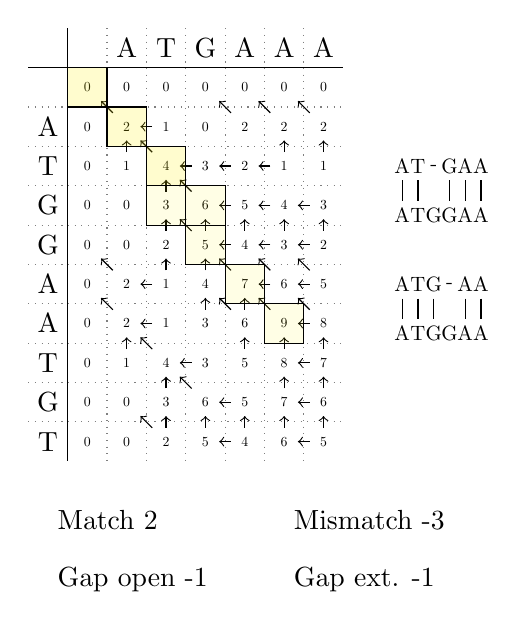
\begin{tikzpicture}[scale=0.5]
      \node [right] at (1,-1) {Match 2};
\node [right] at (7,-1) {Mismatch -3};
\node [right] at (1,-2.5) {Gap open -1};
\node [right] at (7,-2.5) {Gap ext. -1};
\visible<2->{
\draw [-] (0.5,10.5) -- (8.5,10.5);
\draw [-] (1.5,11.5) -- (1.5,0.5);
\draw [-, dotted, opacity=0.5] (0.5,9.5) -- (8.5,9.5);
\draw [-, dotted, opacity=0.5] (2.5,11.5) -- (2.5,0.5);
	\node at (3,11) {A};
	\draw [-, dotted, opacity=0.5] (3.5,11.5) -- (3.5,0.5);
	\node at (4,11) {T};
	\draw [-, dotted, opacity=0.5] (4.5,11.5) -- (4.5,0.5);
	\node at (5,11) {G};
	\draw [-, dotted, opacity=0.5] (5.5,11.5) -- (5.5,0.5);
	\node at (6,11) {A};
	\draw [-, dotted, opacity=0.5] (6.5,11.5) -- (6.5,0.5);
	\node at (7,11) {A};
	\draw [-, dotted, opacity=0.5] (7.5,11.5) -- (7.5,0.5);
	\node at (8,11) {A};
	\node at (1,9) {A};
	\draw [-, dotted, opacity=0.5] (0.5,8.5) -- (8.5,8.5);
	\node at (1,8) {T};
	\draw [-, dotted, opacity=0.5] (0.5,7.5) -- (8.5,7.5);
	\node at (1,7) {G};
	\draw [-, dotted, opacity=0.5] (0.5,6.5) -- (8.5,6.5);
	\node at (1,6) {G};
	\draw [-, dotted, opacity=0.5] (0.5,5.5) -- (8.5,5.5);
	\node at (1,5) {A};
	\draw [-, dotted, opacity=0.5] (0.5,4.5) -- (8.5,4.5);
	\node at (1,4) {A};
	\draw [-, dotted, opacity=0.5] (0.5,3.5) -- (8.5,3.5);
	\node at (1,3) {T};
	\draw [-, dotted, opacity=0.5] (0.5,2.5) -- (8.5,2.5);
	\node at (1,2) {G};
	\draw [-, dotted, opacity=0.5] (0.5,1.5) -- (8.5,1.5);
	\node at (1,1) {T};
}
\visible<3->{
	\node[scale=0.5] at (2,10) {0};
	\node[scale=0.5] at (3,10) {0};
	\node[scale=0.5] at(4,10) {0};
	\node[scale=0.5] at(5,10) {0};
	\node[scale=0.5] at(6,10) {0};
	\node[scale=0.5] at(7,10) {0};
	\node[scale=0.5] at(8,10) {0};
	\node[scale=0.5] at (2,9) {0};
	\node[scale=0.5] at(2,8) {0};
	\node[scale=0.5] at(2,7) {0};
	\node[scale=0.5] at(2,6) {0};
	\node[scale=0.5] at(2,5) {0};
	\node[scale=0.5] at(2,4) {0};
	\node[scale=0.5] at(2,3) {0};
	\node[scale=0.5] at(2,2) {0};
	\node[scale=0.5] at(2,1) {0};
}
\visible<4->{
	\node [scale=0.5] at (3,9) {2};
	\draw [->] (2.65,9.35) -- (2.35,9.65);
	\node [scale=0.5] at (4,9) {1};
	\draw [->] (3.65,9) -- (3.35,9);
	\node [scale=0.5] at (5,9) {0};
	\node [scale=0.5] at (6,9) {2};
	\draw [->] (5.65,9.35) -- (5.35,9.65);
	\node [scale=0.5] at (7,9) {2};
	\draw [->] (6.65,9.35) -- (6.35,9.65);
	\node [scale=0.5] at (8,9) {2};
	\draw [->] (7.65,9.35) -- (7.35,9.65);
}
\visible<5->{
	\node [scale=0.5] at (3,8) {1};
	\draw [->] (3,8.35) -- (3,8.65);
	\node [scale=0.5] at (4,8) {4};
	\draw [->] (3.65,8.35) -- (3.35,8.65);
	\node [scale=0.5] at (5,8) {3};
	\draw [->] (4.65,8) -- (4.35,8);
	\node [scale=0.5] at (6,8) {2};
	\draw [->] (5.65,8) -- (5.35,8);
	\node [scale=0.5] at (7,8) {1};
	\draw [->] (6.65,8) -- (6.35,8);
	\draw [->] (7,8.35) -- (7,8.65);
	\node [scale=0.5] at (8,8) {1};
	\draw [->] (8,8.35) -- (8,8.65);
}
\visible<6->{
	\node [scale=0.5] at (3,7) {0};
	\node [scale=0.5] at (4,7) {3};
	\draw [->] (4,7.35) -- (4,7.65);
	\node [scale=0.5] at (5,7) {6};
	\draw [->] (4.65,7.35) -- (4.35,7.65);
	\node [scale=0.5] at (6,7) {5};
	\draw [->] (5.65,7) -- (5.35,7);
	\node [scale=0.5] at (7,7) {4};
	\draw [->] (6.65,7) -- (6.35,7);
	\node [scale=0.5] at (8,7) {3};
	\draw [->] (7.65,7) -- (7.35,7);
}
\visible<7->{
	\node [scale=0.5] at (3,6) {0};
	\node [scale=0.5] at (4,6) {2};
	\draw [->] (4,6.35) -- (4,6.65);
	\node [scale=0.5] at (5,6) {5};
	\draw [->] (4.65,6.35) -- (4.35,6.65);
	\draw [->] (5,6.35) -- (5,6.65);
	\node [scale=0.5] at (6,6) {4};
	\draw [->] (5.65,6) -- (5.35,6);
	\draw [->] (6,6.35) -- (6,6.65);
	\node [scale=0.5] at (7,6) {3};
	\draw [->] (6.65,6) -- (6.35,6);
	\draw [->] (7,6.35) -- (7,6.65);
	\node [scale=0.5] at (8,6) {2};
	\draw [->] (7.65,6) -- (7.35,6);
	\draw [->] (8,6.35) -- (8,6.65);
}
\visible<8->{
	\node [scale=0.5] at (3,5) {2};
	\draw [->] (2.65,5.35) -- (2.35,5.65);
	\node [scale=0.5] at (4,5) {1};
	\draw [->] (3.65,5) -- (3.35,5);
	\draw [->] (4,5.35) -- (4,5.65);
	\node [scale=0.5] at (5,5) {4};
	\draw [->] (5,5.35) -- (5,5.65);
	\node [scale=0.5] at (6,5) {7};
	\draw [->] (5.65,5.35) -- (5.35,5.65);
	\node [scale=0.5] at (7,5) {6};
	\draw [->] (6.65,5.35) -- (6.35,5.65);
	\draw [->] (6.65,5) -- (6.35,5);
	\node [scale=0.5] at (8,5) {5};
	\draw [->] (7.65,5.35) -- (7.35,5.65);
	\draw [->] (7.65,5) -- (7.35,5);
}
\visible<9->{
	\node [scale=0.5] at (3,4) {2};
	\draw [->] (2.65,4.35) -- (2.35,4.65);
	\node [scale=0.5] at (4,4) {1};
	\draw [->] (3.65,4) -- (3.35,4);
	\node [scale=0.5] at (5,4) {3};
	\draw [->] (5,4.35) -- (5,4.65);
	\node [scale=0.5] at (6,4) {6};
	\draw [->] (5.65,4.35) -- (5.35,4.65);
	\draw [->] (6,4.35) -- (6,4.65);
	\node [scale=0.5] at (7,4) {9};
	\draw [->] (6.65,4.35) -- (6.35,4.65);
	\node [scale=0.5] at (8,4) {8};
	\draw [->] (7.65,4.35) -- (7.35,4.65);
	\draw [->] (7.65,4) -- (7.35,4);
}
\visible<10->{
	\node [scale=0.5] at (3,3) {1};
	\draw [->] (3,3.35) -- (3,3.65);
	\node [scale=0.5] at (4,3) {4};
	\draw [->] (3.65,3.35) -- (3.35,3.65);
	\node [scale=0.5] at (5,3) {3};
	\draw [->] (4.65,3) -- (4.35,3);
	\node [scale=0.5] at (6,3) {5};
	\draw [->] (6,3.35) -- (6,3.65);
	\node [scale=0.5] at (7,3) {8};
	\draw [->] (7,3.35) -- (7,3.65);
	\node [scale=0.5] at (8,3) {7};
	\draw [->] (7.65,3) -- (7.35,3);
	\draw [->] (8,3.35) -- (8,3.65);
}
\visible<11->{
	\node [scale=0.5] at (3,2) {0};
	\node [scale=0.5] at (4,2) {3};
	\draw [->] (4,2.35) -- (4,2.65);
	\node [scale=0.5] at (5,2) {6};
	\draw [->] (4.65,2.35) -- (4.35,2.65);
	\node [scale=0.5] at (6,2) {5};
	\draw [->] (5.65,2) -- (5.35,2);
	\node [scale=0.5] at (7,2) {7};
	\draw [->] (7,2.35) -- (7,2.65);
	\node [scale=0.5] at (8,2) {6};
	\draw [->] (7.65,2) -- (7.35,2);
	\draw [->] (8,2.35) -- (8,2.65);
}
\visible<12->{
	\node [scale=0.5] at (3,1) {0};
	\node [scale=0.5] at (4,1) {2};
	\draw [->] (3.65,1.35) -- (3.35,1.65);
	\draw [->] (4,1.35) -- (4,1.65);
	\node [scale=0.5] at (5,1) {5};
	\draw [->] (5,1.35) -- (5,1.65);
	\node [scale=0.5] at (6,1) {4};
	\draw [->] (5.65,1) -- (5.35,1);
	\draw [->] (6,1.35) -- (6,1.65);
	\node [scale=0.5] at (7,1) {6};
	\draw [->] (7,1.35) -- (7,1.65);
	\node [scale=0.5] at (8,1) {5};
	\draw [->] (7.65,1) -- (7.35,1);
	\draw [->] (8,1.35) -- (8,1.65);
}
\visible<13->{
\draw [fill=yellow, fill opacity=0.1] (6.5,3.5) rectangle (7.5,4.5);
}
\visible<14->{
\draw [fill=yellow, fill opacity=0.1] (5.5,4.5) rectangle (6.5,5.5);
}
\visible<15->{
\draw [fill=yellow, fill opacity=0.1] (4.5,5.5) rectangle (5.5,6.5);
}
\visible<16->{
\draw [fill=yellow, fill opacity=0.1] (3.5,6.5) rectangle (4.5,7.5);
}
\visible<17->{
\draw [fill=yellow, fill opacity=0.1] (3.5,7.5) rectangle (4.5,8.5);
}
\visible<18->{
\draw [fill=yellow, fill opacity=0.1] (2.5,8.5) rectangle (3.5,9.5);
}
\visible<19->{
\draw [fill=yellow, fill opacity=0.1] (1.5,9.5) rectangle (2.5,10.5);
}
\visible<20->{
\draw [fill=yellow, fill opacity=0.1] (4.5,6.5) rectangle (5.5,7.5);
}
\visible<21->{
\draw [fill=yellow, fill opacity=0.1] (3.5,7.5) rectangle (4.5,8.5);
}
\visible<22->{
\draw [fill=yellow, fill opacity=0.1] (2.5,8.5) rectangle (3.5,9.5);
}
\visible<23->{
\draw [fill=yellow, fill opacity=0.1] (1.5,9.5) rectangle (2.5,10.5);
}
\visible<24->{
\node [scale=0.75] (s1) at (10 + 0/2.5, 8) {A};
\node [scale=0.75] (s2) at (10 + 0/2.5, 8-1.25) {A};
\draw [-] (s1) -- (s2);
\node [scale=0.75] (s1) at (10 + 1/2.5, 8) {T};
\node [scale=0.75] (s2) at (10 + 1/2.5, 8-1.25) {T};
\draw [-] (s1) -- (s2);
\node [scale=0.75] (s1) at (10 + 2/2.5, 8) {-};
\node [scale=0.75] (s2) at (10 + 2/2.5, 8-1.25) {G};
\node [scale=0.75] (s1) at (10 + 3/2.5, 8) {G};
\node [scale=0.75] (s2) at (10 + 3/2.5, 8-1.25) {G};
\draw [-] (s1) -- (s2);
\node [scale=0.75] (s1) at (10 + 4/2.5, 8) {A};
\node [scale=0.75] (s2) at (10 + 4/2.5, 8-1.25) {A};
\draw [-] (s1) -- (s2);
\node [scale=0.75] (s1) at (10 + 5/2.5, 8) {A};
\node [scale=0.75] (s2) at (10 + 5/2.5, 8-1.25) {A};
\draw [-] (s1) -- (s2);
\node [scale=0.75] (s1) at (10 + 0/2.5, 5) {A};
\node [scale=0.75] (s2) at (10 + 0/2.5, 5-1.25) {A};
\draw [-] (s1) -- (s2);
\node [scale=0.75] (s1) at (10 + 1/2.5, 5) {T};
\node [scale=0.75] (s2) at (10 + 1/2.5, 5-1.25) {T};
\draw [-] (s1) -- (s2);
\node [scale=0.75] (s1) at (10 + 2/2.5, 5) {G};
\node [scale=0.75] (s2) at (10 + 2/2.5, 5-1.25) {G};
\draw [-] (s1) -- (s2);
\node [scale=0.75] (s1) at (10 + 3/2.5, 5) {-};
\node [scale=0.75] (s2) at (10 + 3/2.5, 5-1.25) {G};
\node [scale=0.75] (s1) at (10 + 4/2.5, 5) {A};
\node [scale=0.75] (s2) at (10 + 4/2.5, 5-1.25) {A};
\draw [-] (s1) -- (s2);
\node [scale=0.75] (s1) at (10 + 5/2.5, 5) {A};
\node [scale=0.75] (s2) at (10 + 5/2.5, 5-1.25) {A};
\draw [-] (s1) -- (s2);
}

    \end{tikzpicture}
  \end{figure}
\end{frame}

\begin{frame}{Smith-Waterman: local alignment (4)}
  \begin{figure}[ht]
    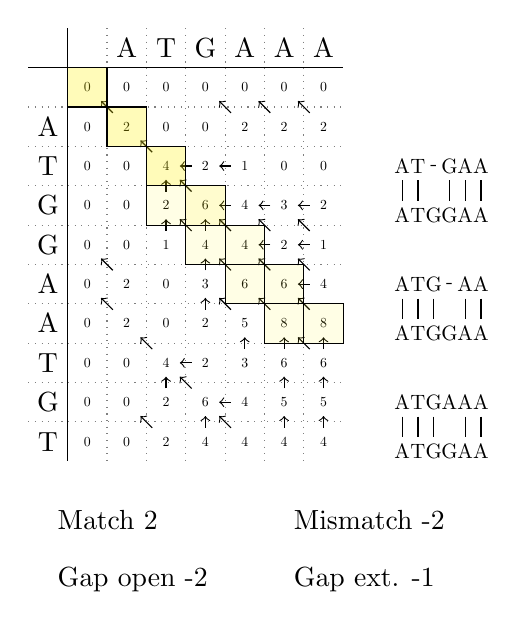
\begin{tikzpicture}[scale=0.5]
      \node [right] at (1,-1) {Match 2};
\node [right] at (7,-1) {Mismatch -2};
\node [right] at (1,-2.5) {Gap open -2};
\node [right] at (7,-2.5) {Gap ext. -1};
\visible<2->{
\draw [-] (0.5,10.5) -- (8.5,10.5);
\draw [-] (1.5,11.5) -- (1.5,0.5);
\draw [-, dotted, opacity=0.5] (0.5,9.5) -- (8.5,9.5);
\draw [-, dotted, opacity=0.5] (2.5,11.5) -- (2.5,0.5);
	\node at (3,11) {A};
	\draw [-, dotted, opacity=0.5] (3.5,11.5) -- (3.5,0.5);
	\node at (4,11) {T};
	\draw [-, dotted, opacity=0.5] (4.5,11.5) -- (4.5,0.5);
	\node at (5,11) {G};
	\draw [-, dotted, opacity=0.5] (5.5,11.5) -- (5.5,0.5);
	\node at (6,11) {A};
	\draw [-, dotted, opacity=0.5] (6.5,11.5) -- (6.5,0.5);
	\node at (7,11) {A};
	\draw [-, dotted, opacity=0.5] (7.5,11.5) -- (7.5,0.5);
	\node at (8,11) {A};
	\node at (1,9) {A};
	\draw [-, dotted, opacity=0.5] (0.5,8.5) -- (8.5,8.5);
	\node at (1,8) {T};
	\draw [-, dotted, opacity=0.5] (0.5,7.5) -- (8.5,7.5);
	\node at (1,7) {G};
	\draw [-, dotted, opacity=0.5] (0.5,6.5) -- (8.5,6.5);
	\node at (1,6) {G};
	\draw [-, dotted, opacity=0.5] (0.5,5.5) -- (8.5,5.5);
	\node at (1,5) {A};
	\draw [-, dotted, opacity=0.5] (0.5,4.5) -- (8.5,4.5);
	\node at (1,4) {A};
	\draw [-, dotted, opacity=0.5] (0.5,3.5) -- (8.5,3.5);
	\node at (1,3) {T};
	\draw [-, dotted, opacity=0.5] (0.5,2.5) -- (8.5,2.5);
	\node at (1,2) {G};
	\draw [-, dotted, opacity=0.5] (0.5,1.5) -- (8.5,1.5);
	\node at (1,1) {T};
}
\visible<3->{
	\node[scale=0.5] at (2,10) {0};
	\node[scale=0.5] at (3,10) {0};
	\node[scale=0.5] at(4,10) {0};
	\node[scale=0.5] at(5,10) {0};
	\node[scale=0.5] at(6,10) {0};
	\node[scale=0.5] at(7,10) {0};
	\node[scale=0.5] at(8,10) {0};
	\node[scale=0.5] at (2,9) {0};
	\node[scale=0.5] at(2,8) {0};
	\node[scale=0.5] at(2,7) {0};
	\node[scale=0.5] at(2,6) {0};
	\node[scale=0.5] at(2,5) {0};
	\node[scale=0.5] at(2,4) {0};
	\node[scale=0.5] at(2,3) {0};
	\node[scale=0.5] at(2,2) {0};
	\node[scale=0.5] at(2,1) {0};
}
\visible<4->{
	\node [scale=0.5] at (3,9) {2};
	\draw [->] (2.65,9.35) -- (2.35,9.65);
	\node [scale=0.5] at (4,9) {0};
	\node [scale=0.5] at (5,9) {0};
	\node [scale=0.5] at (6,9) {2};
	\draw [->] (5.65,9.35) -- (5.35,9.65);
	\node [scale=0.5] at (7,9) {2};
	\draw [->] (6.65,9.35) -- (6.35,9.65);
	\node [scale=0.5] at (8,9) {2};
	\draw [->] (7.65,9.35) -- (7.35,9.65);
}
\visible<5->{
	\node [scale=0.5] at (3,8) {0};
	\node [scale=0.5] at (4,8) {4};
	\draw [->] (3.65,8.35) -- (3.35,8.65);
	\node [scale=0.5] at (5,8) {2};
	\draw [->] (4.65,8) -- (4.35,8);
	\node [scale=0.5] at (6,8) {1};
	\draw [->] (5.65,8) -- (5.35,8);
	\node [scale=0.5] at (7,8) {0};
	\node [scale=0.5] at (8,8) {0};
}
\visible<6->{
	\node [scale=0.5] at (3,7) {0};
	\node [scale=0.5] at (4,7) {2};
	\draw [->] (4,7.35) -- (4,7.65);
	\node [scale=0.5] at (5,7) {6};
	\draw [->] (4.65,7.35) -- (4.35,7.65);
	\node [scale=0.5] at (6,7) {4};
	\draw [->] (5.65,7) -- (5.35,7);
	\node [scale=0.5] at (7,7) {3};
	\draw [->] (6.65,7) -- (6.35,7);
	\node [scale=0.5] at (8,7) {2};
	\draw [->] (7.65,7) -- (7.35,7);
}
\visible<7->{
	\node [scale=0.5] at (3,6) {0};
	\node [scale=0.5] at (4,6) {1};
	\draw [->] (4,6.35) -- (4,6.65);
	\node [scale=0.5] at (5,6) {4};
	\draw [->] (4.65,6.35) -- (4.35,6.65);
	\draw [->] (5,6.35) -- (5,6.65);
	\node [scale=0.5] at (6,6) {4};
	\draw [->] (5.65,6.35) -- (5.35,6.65);
	\node [scale=0.5] at (7,6) {2};
	\draw [->] (6.65,6.35) -- (6.35,6.65);
	\draw [->] (6.65,6) -- (6.35,6);
	\node [scale=0.5] at (8,6) {1};
	\draw [->] (7.65,6.35) -- (7.35,6.65);
	\draw [->] (7.65,6) -- (7.35,6);
}
\visible<8->{
	\node [scale=0.5] at (3,5) {2};
	\draw [->] (2.65,5.35) -- (2.35,5.65);
	\node [scale=0.5] at (4,5) {0};
	\node [scale=0.5] at (5,5) {3};
	\draw [->] (5,5.35) -- (5,5.65);
	\node [scale=0.5] at (6,5) {6};
	\draw [->] (5.65,5.35) -- (5.35,5.65);
	\node [scale=0.5] at (7,5) {6};
	\draw [->] (6.65,5.35) -- (6.35,5.65);
	\node [scale=0.5] at (8,5) {4};
	\draw [->] (7.65,5.35) -- (7.35,5.65);
	\draw [->] (7.65,5) -- (7.35,5);
}
\visible<9->{
	\node [scale=0.5] at (3,4) {2};
	\draw [->] (2.65,4.35) -- (2.35,4.65);
	\node [scale=0.5] at (4,4) {0};
	\node [scale=0.5] at (5,4) {2};
	\draw [->] (5,4.35) -- (5,4.65);
	\node [scale=0.5] at (6,4) {5};
	\draw [->] (5.65,4.35) -- (5.35,4.65);
	\node [scale=0.5] at (7,4) {8};
	\draw [->] (6.65,4.35) -- (6.35,4.65);
	\node [scale=0.5] at (8,4) {8};
	\draw [->] (7.65,4.35) -- (7.35,4.65);
}
\visible<10->{
	\node [scale=0.5] at (3,3) {0};
	\node [scale=0.5] at (4,3) {4};
	\draw [->] (3.65,3.35) -- (3.35,3.65);
	\node [scale=0.5] at (5,3) {2};
	\draw [->] (4.65,3) -- (4.35,3);
	\node [scale=0.5] at (6,3) {3};
	\draw [->] (6,3.35) -- (6,3.65);
	\node [scale=0.5] at (7,3) {6};
	\draw [->] (7,3.35) -- (7,3.65);
	\node [scale=0.5] at (8,3) {6};
	\draw [->] (7.65,3.35) -- (7.35,3.65);
	\draw [->] (8,3.35) -- (8,3.65);
}
\visible<11->{
	\node [scale=0.5] at (3,2) {0};
	\node [scale=0.5] at (4,2) {2};
	\draw [->] (4,2.35) -- (4,2.65);
	\node [scale=0.5] at (5,2) {6};
	\draw [->] (4.65,2.35) -- (4.35,2.65);
	\node [scale=0.5] at (6,2) {4};
	\draw [->] (5.65,2) -- (5.35,2);
	\node [scale=0.5] at (7,2) {5};
	\draw [->] (7,2.35) -- (7,2.65);
	\node [scale=0.5] at (8,2) {5};
	\draw [->] (8,2.35) -- (8,2.65);
}
\visible<12->{
	\node [scale=0.5] at (3,1) {0};
	\node [scale=0.5] at (4,1) {2};
	\draw [->] (3.65,1.35) -- (3.35,1.65);
	\node [scale=0.5] at (5,1) {4};
	\draw [->] (5,1.35) -- (5,1.65);
	\node [scale=0.5] at (6,1) {4};
	\draw [->] (5.65,1.35) -- (5.35,1.65);
	\node [scale=0.5] at (7,1) {4};
	\draw [->] (7,1.35) -- (7,1.65);
	\node [scale=0.5] at (8,1) {4};
	\draw [->] (8,1.35) -- (8,1.65);
}
\visible<13->{
\draw [fill=yellow, fill opacity=0.1] (6.5,3.5) rectangle (7.5,4.5);
}
\visible<14->{
\draw [fill=yellow, fill opacity=0.1] (5.5,4.5) rectangle (6.5,5.5);
}
\visible<15->{
\draw [fill=yellow, fill opacity=0.1] (4.5,5.5) rectangle (5.5,6.5);
}
\visible<16->{
\draw [fill=yellow, fill opacity=0.1] (3.5,6.5) rectangle (4.5,7.5);
}
\visible<17->{
\draw [fill=yellow, fill opacity=0.1] (3.5,7.5) rectangle (4.5,8.5);
}
\visible<18->{
\draw [fill=yellow, fill opacity=0.1] (2.5,8.5) rectangle (3.5,9.5);
}
\visible<19->{
\draw [fill=yellow, fill opacity=0.1] (1.5,9.5) rectangle (2.5,10.5);
}
\visible<20->{
\draw [fill=yellow, fill opacity=0.1] (4.5,6.5) rectangle (5.5,7.5);
}
\visible<21->{
\draw [fill=yellow, fill opacity=0.1] (3.5,7.5) rectangle (4.5,8.5);
}
\visible<22->{
\draw [fill=yellow, fill opacity=0.1] (2.5,8.5) rectangle (3.5,9.5);
}
\visible<23->{
\draw [fill=yellow, fill opacity=0.1] (1.5,9.5) rectangle (2.5,10.5);
}
\visible<24->{
\draw [fill=yellow, fill opacity=0.1] (7.5,3.5) rectangle (8.5,4.5);
}
\visible<25->{
\draw [fill=yellow, fill opacity=0.1] (6.5,4.5) rectangle (7.5,5.5);
}
\visible<26->{
\draw [fill=yellow, fill opacity=0.1] (5.5,5.5) rectangle (6.5,6.5);
}
\visible<27->{
\draw [fill=yellow, fill opacity=0.1] (4.5,6.5) rectangle (5.5,7.5);
}
\visible<28->{
\draw [fill=yellow, fill opacity=0.1] (3.5,7.5) rectangle (4.5,8.5);
}
\visible<29->{
\draw [fill=yellow, fill opacity=0.1] (2.5,8.5) rectangle (3.5,9.5);
}
\visible<30->{
\draw [fill=yellow, fill opacity=0.1] (1.5,9.5) rectangle (2.5,10.5);
}
\visible<31->{
\node [scale=0.75] (s1) at (10 + 0/2.5, 8) {A};
\node [scale=0.75] (s2) at (10 + 0/2.5, 8-1.25) {A};
\draw [-] (s1) -- (s2);
\node [scale=0.75] (s1) at (10 + 1/2.5, 8) {T};
\node [scale=0.75] (s2) at (10 + 1/2.5, 8-1.25) {T};
\draw [-] (s1) -- (s2);
\node [scale=0.75] (s1) at (10 + 2/2.5, 8) {-};
\node [scale=0.75] (s2) at (10 + 2/2.5, 8-1.25) {G};
\node [scale=0.75] (s1) at (10 + 3/2.5, 8) {G};
\node [scale=0.75] (s2) at (10 + 3/2.5, 8-1.25) {G};
\draw [-] (s1) -- (s2);
\node [scale=0.75] (s1) at (10 + 4/2.5, 8) {A};
\node [scale=0.75] (s2) at (10 + 4/2.5, 8-1.25) {A};
\draw [-] (s1) -- (s2);
\node [scale=0.75] (s1) at (10 + 5/2.5, 8) {A};
\node [scale=0.75] (s2) at (10 + 5/2.5, 8-1.25) {A};
\draw [-] (s1) -- (s2);
\node [scale=0.75] (s1) at (10 + 0/2.5, 5) {A};
\node [scale=0.75] (s2) at (10 + 0/2.5, 5-1.25) {A};
\draw [-] (s1) -- (s2);
\node [scale=0.75] (s1) at (10 + 1/2.5, 5) {T};
\node [scale=0.75] (s2) at (10 + 1/2.5, 5-1.25) {T};
\draw [-] (s1) -- (s2);
\node [scale=0.75] (s1) at (10 + 2/2.5, 5) {G};
\node [scale=0.75] (s2) at (10 + 2/2.5, 5-1.25) {G};
\draw [-] (s1) -- (s2);
\node [scale=0.75] (s1) at (10 + 3/2.5, 5) {-};
\node [scale=0.75] (s2) at (10 + 3/2.5, 5-1.25) {G};
\node [scale=0.75] (s1) at (10 + 4/2.5, 5) {A};
\node [scale=0.75] (s2) at (10 + 4/2.5, 5-1.25) {A};
\draw [-] (s1) -- (s2);
\node [scale=0.75] (s1) at (10 + 5/2.5, 5) {A};
\node [scale=0.75] (s2) at (10 + 5/2.5, 5-1.25) {A};
\draw [-] (s1) -- (s2);
\node [scale=0.75] (s1) at (10 + 0/2.5, 2) {A};
\node [scale=0.75] (s2) at (10 + 0/2.5, 2-1.25) {A};
\draw [-] (s1) -- (s2);
\node [scale=0.75] (s1) at (10 + 1/2.5, 2) {T};
\node [scale=0.75] (s2) at (10 + 1/2.5, 2-1.25) {T};
\draw [-] (s1) -- (s2);
\node [scale=0.75] (s1) at (10 + 2/2.5, 2) {G};
\node [scale=0.75] (s2) at (10 + 2/2.5, 2-1.25) {G};
\draw [-] (s1) -- (s2);
\node [scale=0.75] (s1) at (10 + 3/2.5, 2) {A};
\node [scale=0.75] (s2) at (10 + 3/2.5, 2-1.25) {G};
\node [scale=0.75] (s1) at (10 + 4/2.5, 2) {A};
\node [scale=0.75] (s2) at (10 + 4/2.5, 2-1.25) {A};
\draw [-] (s1) -- (s2);
\node [scale=0.75] (s1) at (10 + 5/2.5, 2) {A};
\node [scale=0.75] (s2) at (10 + 5/2.5, 2-1.25) {A};
\draw [-] (s1) -- (s2);
}

    \end{tikzpicture}
  \end{figure}
\end{frame}


\begin{frame}{The penalties}
  Match vs. mismatch vs gap insertion vs gap extension.
  
  Only relative values matter.\\ 
  Determined by:
  
  \begin{itemize}
  \item Frequency of substitution vs / insertion-deletion mutations
  \item Objective of alignment (evolutionary vs functional
    homology\footnote{This term may be a little contentious and conflict with
      common usage.}),
  and type of sequence (DNA / Protein). 
  \end{itemize}

  \pause
  Consider:
  \begin{itemize}
  \item The modular structure of proteins where functional domains
    can be separated by non-conserved loops which may have arisen
    through genetic rearrangements.
  \item Regulatory elements where a short separation can be tolerated.
  \item Exons separated by variable length introns.
  \end{itemize}

\end{frame}

\begin{frame}{The penalties (2)}
  Typical values:\footnote{taken from \url{https://blast.ncbi.nlm.nih.gov/Blast.cgi?PAGE_TYPE=BlastSearch&PROG_DEF=blastn&BLAST_PROG_DEF=blastn&BLAST_SPEC=GlobalAln&LINK_LOC=BlastHomeLink}}
  \begin{description}[Gap Extension]
  \item[Match] +2
  \item[Mismatch] -3
  \item[Gap Insertion] -5
  \item[Gap Extension] -2
  \end{description}

  But larger gap insertion penalties are common.
  \vspace{0.2cm}
  Penalty / score / cost can all refer to the same thing, but with different signs.
  
\end{frame}

\begin{frame}{Nucleotide substitutions}
  In the above equations we have used a single mismatch penalty for all
  nucleotide substitutions. However (at least) two types exist:
 
 \vspace{0.2cm}
  \begin{description}[Transversion]
  \item[Transition] purine $\Leftrightarrow$ purine \\ pyrimidine
    $\Leftrightarrow$ pyrimidine
  \item[Transversion] pyrimidine $\Leftrightarrow$ purine
  \end{description}
    
  Transversion less likely, and should infer a greater penalty.

\end{frame}

\begin{frame}{A nucleotide substitution matrix}
  \begin{columns}[t]
    \begin{column}{0.5\textwidth}
      \begin{tabular}{ c| c c c c }
        & \textcolor{pur}{A} & \textcolor{pyr}{C} & \textcolor{pyr}{T} & \textcolor{pur}{G}\\
        \hline
        \textcolor{pur}{A} & 1 \\
        \textcolor{pyr}{C} & -2& 1 \\
        \textcolor{pyr}{T} & -2& -1& 1\\
        \textcolor{pur}{G} & -1& -2& -1& 1\\
      \end{tabular}
    \end{column}
    \begin{column}{0.5\textwidth}
      \begin{tabular}{ c c c l }
        \multicolumn{3}{c}{mutation} & cost \\
        \textcolor{pyr}{C} & $\Leftrightarrow$ & \textcolor{pur}{A} & -2 \\
        \textcolor{pyr}{T} & $\Leftrightarrow$ & \textcolor{pur}{A} & -2 \\
        \textcolor{pyr}{T} & $\Leftrightarrow$ & \textcolor{pyr}{C} & -1 \\
        \textcolor{pur}{G} & $\Leftrightarrow$ & \textcolor{pur}{A} & -1 \\
        \textcolor{pur}{G} & $\Leftrightarrow$ & \textcolor{pyr}{C} & -2 \\
        \textcolor{pur}{G} & $\Leftrightarrow$ & \textcolor{pyr}{T} & -1 \\
      \end{tabular}
    \end{column}
  \end{columns}
  \textcolor{pur}{Purine}\\
  \textcolor{pyr}{Pyrimidine}

  Suriprisingly however, the identity matrix is almost always used. So the
  above is not that useful.
\end{frame}

\begin{frame}{Protein substitution matrices}
  20 amino acids with widely different properties.
  Substitution matrices:
  {\small
  \begin{itemize}
  \item Mutation distances. Based on the number of DNA base changes required to convert
    codons. (Fitch substitution model)
  \item Chemical properties. Based on chemical properties of amino acids
    (size, hydrophobicity, charge, pH). Dissimilar amino acids incur larger costs.
  \item Evolutionary tendencies. Based on the frequency of mutation within
    homologous proteins. Infrequently observed changes incur greater costs.
    \begin{description}
    \item[PAM] Percentage of Acceptable point Mutations. Based on global alignments of closely
      related proteins. (Dayhoff et al.)
    \item[BLOSUM] Blocks Substitution Matrix. Based on local alignmens from the
      Blocks database. Based on a larger set of proteins than PAM. (Henikoff \& Henikoff)
      sensitive.
    \end{description}
  \end{itemize}
  }
\end{frame}

\begin{frame}{Protein substitution matrices (2)}
  PAM \& BLOSUM are the predominantly used families of matrices.

  Which to use depends on specific situation. For more divergent sequences
  use highly numbered PAM matrices, but low numbered Blosum matrices.

  In general, use the default set by the program used, unless you know
  better.\\
  No clear answers to the question. 

  For more information see:\\
  \url{http://www.ctu.edu.vn/~dvxe/Bioinformatic\%20course/mod4/mod4_0.html}
  
\end{frame}

\begin{frame}{PAM 256}
  \begin{figure}[ht]
    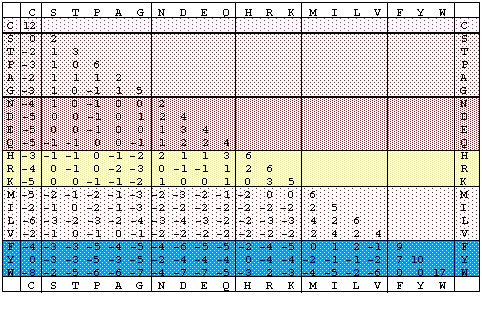
\includegraphics[width=0.6\textwidth]{images/dayhoff_256}
    \caption{  PAM 256 (aka Dayhoff 256) substitution matrix. Amino acids are
    grouped by the chemistry of their side group.}
  \end{figure}
  \blfootnote{Image taken from:
    \url{http://www.ctu.edu.vn/~dvxe/Bioinformatic\%20course/mod4/mod4_0.html}.\\
  But many copies on the web, unsure of original.}
\end{frame}

\begin{frame}{Protein or Nucleotide}
  From a computational point of view it doesn't matter whether aligning
  protein or DNA sequences. 

  Just a question of changing the parameters and the
  substitution matrices to suit the question at hand.

\end{frame}

\begin{frame}{Homology and Similarity}
  \textcolor{navy}{\emph{Homology implies}} either an evolutionary or functional
  relationship. Nucleotides or amino acids within a homologous
  region may be considered as homologous.

  Regions of homology can be identified when they have a \textcolor{navy}{\emph{similarity}}
  larger than that expected by chance.

  Functional homology in protein sequences (probably) mostly arise
  from evolutionary homology (i.e. not convergent evolution).

  Functional homology\footnote{Again, be careful with this phrase!} in regulatory elements is more likely to arise through
  convergent evolution as the sequence requirements are much less stringent.
  Such homology though is difficult to identify in the absence of evolutionary
  homology due to low information content.
  
\end{frame}

\begin{frame}{Implementations}
  Easy to find. Use Google.
  \begin{description}
  \item[EBI] \url{http://www.ebi.ac.uk/Tools/psa/}
  \item[NCBI]
    \url{https://blast.ncbi.nlm.nih.gov/Blast.cgi?PAGE_TYPE=BlastSearch\&PROG_DEF=blastn\&BLAST_PROG_DEF=blastn\&BLAST_SPEC=GlobalAln&LINK_LOC=BlastHomeLink}
  \end{description}
\end{frame}

\begin{frame}{Perl to Latex}
  I implemented the Needleman-Wunsch and Smith-Waterman algorithms in Perl to make
  these slides.

  Good for playing around with parameters to get a good understanding
  of the algorithms. Easy to modify.

  I will clean up the code and make it available on Fronter if anyone has an interest?
\end{frame}

\end{document}
